\documentclass[11pt]{article}

% Overleaf: tải cả thư mục report/ lên (đã có acl.sty, acl_natbib.bst, custom.bib, figures/, sections/),
% Menu -> Settings -> Compiler: XeLaTeX. Trang chính: main.tex.

% ACL official style
\usepackage[final]{acl}

% Standard packages
\usepackage{microtype}
\usepackage{graphicx}
\usepackage{booktabs}
\usepackage{multirow}
\usepackage{xcolor}
\usepackage{tikz}
\usetikzlibrary{positioning,arrows.meta}

% Vietnamese support - XeLaTeX
\usepackage{fontspec}
\setmainfont{TeX Gyre Termes}

\renewcommand{\tablename}{Bảng}
\renewcommand{\figurename}{Hình}
\renewcommand{\refname}{Tài liệu tham khảo}
\renewcommand{\abstractname}{Tóm tắt}

\title{Phát hiện biển báo giao thông Việt Nam trên ảnh camera hành trình:\\
So sánh YOLOv8 và Faster R-CNN với biển báo nhỏ\\
(Báo cáo cuối kỳ -- Nhóm 19)}

\author{
Hoàng Hải Anh \\ 24022248
\And
Tạ Mạnh Cường \\ 24022278
\And
Phạm Thế Hưng \\ 24022350
\AND
Học sâu -- GV: Nguyễn Việt Hà \\
Trường Đại học Công nghệ, ĐHQGHN
}

\begin{document}

\maketitle

\begin{abstract}
Nhóm so sánh mô hình một giai đoạn YOLOv8 và mô hình hai giai đoạn Faster R-CNN ResNet50-FPN cho bài toán phát hiện 7 loại biển báo giao thông trên ảnh camera hành trình Việt Nam (Zalo AI 2020). Trong bộ dữ liệu này, 77,6\% biển có diện tích dưới $32^2$ pixel.
Trước khi huấn luyện, nhóm gộp 17,5\% box bị gán lặp và chia tập theo tuyến đường để tránh rò rỉ dữ liệu.
Trên tập test, YOLOv8s ở kích thước đầu vào 1280 đạt 76,8 mAP@0.5, cao hơn Faster R-CNN 7,5 điểm (có ý nghĩa thống kê theo bootstrap), và suy luận nhanh hơn 5,8 lần (71 so với 12 FPS trên GPU T4).
Giữ độ phân giải, bằng cách tăng kích thước đầu vào hoặc cắt ô kết hợp SAHI, làm AP với biển nhỏ tăng khoảng 20 điểm.
Phân tích lỗi cho thấy:
(i) phần lớn lỗi là bỏ sót biển dưới 16 pixel;
(ii) nhầm lớp tập trung ở ba lớp biển tròn viền đỏ, và cân bằng lớp bằng oversampling hay trọng số lớp chỉ chuyển lỗi giữa các lớp này;
(iii) chia tập ngẫu nhiên làm điểm cao hơn thực tế 5,7 điểm.
\end{abstract}

% ------------------------------------------------
% GIỚI THIỆU. Ghép vào báo cáo chính bằng % ------------------------------------------------
% GIỚI THIỆU. Ghép vào báo cáo chính bằng % ------------------------------------------------
% GIỚI THIỆU. Ghép vào báo cáo chính bằng \input{sections/intro}
% ------------------------------------------------

\section{Giới thiệu}
\label{sec:intro}

Phát hiện biển báo giao thông là một thành phần của các hệ thống hỗ trợ lái xe (ADAS) và xe tự hành.
Với camera hành trình góc rộng trên đường phố Việt Nam, bài toán có ba khó khăn đặc thù.
Thứ nhất, phần lớn biển báo ở xa nên rất nhỏ so với khung hình.
Thứ hai, nhiều biển được gắn sát nhau trên cùng một cột.
Thứ ba, số lượng mẫu giữa các loại biển chênh lệch nhau.

\paragraph{Bài toán.}
Đầu vào là một ảnh RGB $1622 \times 626$ chụp từ camera hành trình.
Đầu ra là danh sách các phát hiện $(b_i, c_i, s_i)$, trong đó $b_i = [x, y, w, h]$ là hộp bao tính bằng pixel trên ảnh gốc, $c_i$ là một trong 7 lớp biển báo, và $s_i \in [0, 1]$ là độ tin cậy.
Nhóm dùng bộ dữ liệu Zalo AI Challenge 2020 \citep{zalo2020traffic}, gồm 4.500 ảnh có nhãn.
Ở bộ dữ liệu này, 77,6\% biển có diện tích dưới $32^2$ pixel, và cạnh trung vị chỉ 16,5 pixel.

\paragraph{Câu hỏi nghiên cứu.}
Nhóm so sánh hai trường phái phát hiện đối tượng tiêu biểu: YOLOv8 một giai đoạn \citep{jocher2023ultralytics} và Faster R-CNN hai giai đoạn với FPN \citep{ren2015faster,lin2017fpn}.
Câu hỏi đặt ra là trên dữ liệu có nhiều biển nhỏ: (i) họ mô hình nào chính xác hơn và nhanh hơn; (ii) cách xử lý biển nhỏ nào hiệu quả; (iii) lỗi còn lại đến từ đâu.

\paragraph{Đóng góp.}
\begin{itemize}
\item \textbf{Làm sạch dữ liệu và giao thức đánh giá.} Nhóm phát hiện và gộp 17,5\% box bị gán lặp. Nếu giữ nguyên, recall tối đa trên tập test chỉ khoảng 77\%. Nhóm chia tập theo tuyến đường, và dùng chung một script đánh giá cho mọi mô hình, kèm kiểm định bootstrap.
\item \textbf{So sánh hai họ mô hình trên cùng giao thức.} Trên tập test, YOLOv8s ở imgsz 1280 đạt 76,8 mAP@0.5. Con số này cao hơn Faster R-CNN ResNet50-FPN 7,5 điểm (có ý nghĩa thống kê), trong khi suy luận nhanh hơn khoảng 6 lần trên cùng GPU.
\item \textbf{Phân tích lỗi.} Lỗi chính là bỏ sót biển nhỏ: 87--92\% số biển bị bỏ sót có kích thước dưới 16 pixel. Nhầm lớp chủ yếu xảy ra giữa ba lớp biển tròn viền đỏ. Nhãn test vẫn còn biển thiếu nhãn và nhãn sai lớp.
\item \textbf{Hai thí nghiệm phân tích.} (i) Chia tập ngẫu nhiên làm điểm trên val cao hơn thực tế 5,7 điểm. (ii) Cân bằng lớp bằng oversampling hoặc trọng số lớp không cải thiện các lớp hiếm, và nhóm chỉ ra vì sao.
\end{itemize}

% ------------------------------------------------

\section{Giới thiệu}
\label{sec:intro}

Phát hiện biển báo giao thông là một thành phần của các hệ thống hỗ trợ lái xe (ADAS) và xe tự hành.
Với camera hành trình góc rộng trên đường phố Việt Nam, bài toán có ba khó khăn đặc thù.
Thứ nhất, phần lớn biển báo ở xa nên rất nhỏ so với khung hình.
Thứ hai, nhiều biển được gắn sát nhau trên cùng một cột.
Thứ ba, số lượng mẫu giữa các loại biển chênh lệch nhau.

\paragraph{Bài toán.}
Đầu vào là một ảnh RGB $1622 \times 626$ chụp từ camera hành trình.
Đầu ra là danh sách các phát hiện $(b_i, c_i, s_i)$, trong đó $b_i = [x, y, w, h]$ là hộp bao tính bằng pixel trên ảnh gốc, $c_i$ là một trong 7 lớp biển báo, và $s_i \in [0, 1]$ là độ tin cậy.
Nhóm dùng bộ dữ liệu Zalo AI Challenge 2020 \citep{zalo2020traffic}, gồm 4.500 ảnh có nhãn.
Ở bộ dữ liệu này, 77,6\% biển có diện tích dưới $32^2$ pixel, và cạnh trung vị chỉ 16,5 pixel.

\paragraph{Câu hỏi nghiên cứu.}
Nhóm so sánh hai trường phái phát hiện đối tượng tiêu biểu: YOLOv8 một giai đoạn \citep{jocher2023ultralytics} và Faster R-CNN hai giai đoạn với FPN \citep{ren2015faster,lin2017fpn}.
Câu hỏi đặt ra là trên dữ liệu có nhiều biển nhỏ: (i) họ mô hình nào chính xác hơn và nhanh hơn; (ii) cách xử lý biển nhỏ nào hiệu quả; (iii) lỗi còn lại đến từ đâu.

\paragraph{Đóng góp.}
\begin{itemize}
\item \textbf{Làm sạch dữ liệu và giao thức đánh giá.} Nhóm phát hiện và gộp 17,5\% box bị gán lặp. Nếu giữ nguyên, recall tối đa trên tập test chỉ khoảng 77\%. Nhóm chia tập theo tuyến đường, và dùng chung một script đánh giá cho mọi mô hình, kèm kiểm định bootstrap.
\item \textbf{So sánh hai họ mô hình trên cùng giao thức.} Trên tập test, YOLOv8s ở imgsz 1280 đạt 76,8 mAP@0.5. Con số này cao hơn Faster R-CNN ResNet50-FPN 7,5 điểm (có ý nghĩa thống kê), trong khi suy luận nhanh hơn khoảng 6 lần trên cùng GPU.
\item \textbf{Phân tích lỗi.} Lỗi chính là bỏ sót biển nhỏ: 87--92\% số biển bị bỏ sót có kích thước dưới 16 pixel. Nhầm lớp chủ yếu xảy ra giữa ba lớp biển tròn viền đỏ. Nhãn test vẫn còn biển thiếu nhãn và nhãn sai lớp.
\item \textbf{Hai thí nghiệm phân tích.} (i) Chia tập ngẫu nhiên làm điểm trên val cao hơn thực tế 5,7 điểm. (ii) Cân bằng lớp bằng oversampling hoặc trọng số lớp không cải thiện các lớp hiếm, và nhóm chỉ ra vì sao.
\end{itemize}

% ------------------------------------------------

\section{Giới thiệu}
\label{sec:intro}

Phát hiện biển báo giao thông là một thành phần của các hệ thống hỗ trợ lái xe (ADAS) và xe tự hành.
Với camera hành trình góc rộng trên đường phố Việt Nam, bài toán có ba khó khăn đặc thù.
Thứ nhất, phần lớn biển báo ở xa nên rất nhỏ so với khung hình.
Thứ hai, nhiều biển được gắn sát nhau trên cùng một cột.
Thứ ba, số lượng mẫu giữa các loại biển chênh lệch nhau.

\paragraph{Bài toán.}
Đầu vào là một ảnh RGB $1622 \times 626$ chụp từ camera hành trình.
Đầu ra là danh sách các phát hiện $(b_i, c_i, s_i)$, trong đó $b_i = [x, y, w, h]$ là hộp bao tính bằng pixel trên ảnh gốc, $c_i$ là một trong 7 lớp biển báo, và $s_i \in [0, 1]$ là độ tin cậy.
Nhóm dùng bộ dữ liệu Zalo AI Challenge 2020 \citep{zalo2020traffic}, gồm 4.500 ảnh có nhãn.
Ở bộ dữ liệu này, 77,6\% biển có diện tích dưới $32^2$ pixel, và cạnh trung vị chỉ 16,5 pixel.

\paragraph{Câu hỏi nghiên cứu.}
Nhóm so sánh hai trường phái phát hiện đối tượng tiêu biểu: YOLOv8 một giai đoạn \citep{jocher2023ultralytics} và Faster R-CNN hai giai đoạn với FPN \citep{ren2015faster,lin2017fpn}.
Câu hỏi đặt ra là trên dữ liệu có nhiều biển nhỏ: (i) họ mô hình nào chính xác hơn và nhanh hơn; (ii) cách xử lý biển nhỏ nào hiệu quả; (iii) lỗi còn lại đến từ đâu.

\paragraph{Đóng góp.}
\begin{itemize}
\item \textbf{Làm sạch dữ liệu và giao thức đánh giá.} Nhóm phát hiện và gộp 17,5\% box bị gán lặp. Nếu giữ nguyên, recall tối đa trên tập test chỉ khoảng 77\%. Nhóm chia tập theo tuyến đường, và dùng chung một script đánh giá cho mọi mô hình, kèm kiểm định bootstrap.
\item \textbf{So sánh hai họ mô hình trên cùng giao thức.} Trên tập test, YOLOv8s ở imgsz 1280 đạt 76,8 mAP@0.5. Con số này cao hơn Faster R-CNN ResNet50-FPN 7,5 điểm (có ý nghĩa thống kê), trong khi suy luận nhanh hơn khoảng 6 lần trên cùng GPU.
\item \textbf{Phân tích lỗi.} Lỗi chính là bỏ sót biển nhỏ: 87--92\% số biển bị bỏ sót có kích thước dưới 16 pixel. Nhầm lớp chủ yếu xảy ra giữa ba lớp biển tròn viền đỏ. Nhãn test vẫn còn biển thiếu nhãn và nhãn sai lớp.
\item \textbf{Hai thí nghiệm phân tích.} (i) Chia tập ngẫu nhiên làm điểm trên val cao hơn thực tế 5,7 điểm. (ii) Cân bằng lớp bằng oversampling hoặc trọng số lớp không cải thiện các lớp hiếm, và nhóm chỉ ra vì sao.
\end{itemize}

% ------------------------------------------------
% CÁC CÔNG TRÌNH LIÊN QUAN. Ghép vào báo cáo chính bằng % ------------------------------------------------
% CÁC CÔNG TRÌNH LIÊN QUAN. Ghép vào báo cáo chính bằng % ------------------------------------------------
% CÁC CÔNG TRÌNH LIÊN QUAN. Ghép vào báo cáo chính bằng \input{sections/related}
% ------------------------------------------------

\section{Các công trình liên quan}
\label{sec:related}

\paragraph{Phát hiện đối tượng một và hai giai đoạn.}
Faster R-CNN \citep{ren2015faster} là mô hình hai giai đoạn. Mạng đề xuất vùng (RPN) sinh ra các vùng có thể chứa vật thể từ một tập anchor định sẵn. Sau đó một đầu RoI phân loại và tinh chỉnh tọa độ cho từng vùng.
YOLO \citep{redmon2016yolo} đưa bài toán về một phép hồi quy duy nhất trên lưới, chỉ cần một lần chạy qua mạng, nên nhanh hơn nhiều.
YOLOv8 \citep{jocher2023ultralytics}, phiên bản nhóm sử dụng, không dùng anchor: mỗi điểm trên bản đồ đặc trưng dự đoán trực tiếp khoảng cách tới bốn cạnh của hộp bao. YOLOv8 cũng tách riêng nhánh phân loại và nhánh hồi quy.

\paragraph{Phát hiện vật thể nhỏ.}
Các mạng CNN giảm dần độ phân giải qua các tầng, nên vật thể nhỏ gần như biến mất ở tầng sâu.
FPN \citep{lin2017fpn} thêm một đường từ trên xuống, đưa ngữ nghĩa của tầng sâu xuống các tầng có độ phân giải cao. Mỗi tầng phụ trách vật thể có kích thước tương ứng, và FPN cải thiện nhiều nhất ở vật thể nhỏ.
Phần neck của YOLOv8 cũng là một kim tự tháp đặc trưng (kiểu PAN). Tuy nhiên, tầng đầu ra mịn nhất có stride 8.
Một hướng khác là giữ nguyên độ phân giải ảnh: SAHI \citep{akyon2022sahi} cắt ảnh thành các ô chồng lấp, dự đoán trên từng ô rồi gộp kết quả.

\paragraph{Mất cân bằng lớp và rò rỉ dữ liệu.}
Với dữ liệu có phân bố đuôi dài, Repeat Factor Sampling \citep{gupta2019lvis} lặp lại các ảnh chứa lớp hiếm khi huấn luyện. Trọng số lớp trong hàm mất mát là cách phổ biến khác.
Rò rỉ dữ liệu xảy ra khi thông tin từ tập đánh giá lọt vào quá trình huấn luyện, khiến kết quả cao hơn thực tế. Với ảnh trích từ video, các khung hình liên tiếp gần như giống hệt nhau là một nguồn rò rỉ điển hình.

% ------------------------------------------------

\section{Các công trình liên quan}
\label{sec:related}

\paragraph{Phát hiện đối tượng một và hai giai đoạn.}
Faster R-CNN \citep{ren2015faster} là mô hình hai giai đoạn. Mạng đề xuất vùng (RPN) sinh ra các vùng có thể chứa vật thể từ một tập anchor định sẵn. Sau đó một đầu RoI phân loại và tinh chỉnh tọa độ cho từng vùng.
YOLO \citep{redmon2016yolo} đưa bài toán về một phép hồi quy duy nhất trên lưới, chỉ cần một lần chạy qua mạng, nên nhanh hơn nhiều.
YOLOv8 \citep{jocher2023ultralytics}, phiên bản nhóm sử dụng, không dùng anchor: mỗi điểm trên bản đồ đặc trưng dự đoán trực tiếp khoảng cách tới bốn cạnh của hộp bao. YOLOv8 cũng tách riêng nhánh phân loại và nhánh hồi quy.

\paragraph{Phát hiện vật thể nhỏ.}
Các mạng CNN giảm dần độ phân giải qua các tầng, nên vật thể nhỏ gần như biến mất ở tầng sâu.
FPN \citep{lin2017fpn} thêm một đường từ trên xuống, đưa ngữ nghĩa của tầng sâu xuống các tầng có độ phân giải cao. Mỗi tầng phụ trách vật thể có kích thước tương ứng, và FPN cải thiện nhiều nhất ở vật thể nhỏ.
Phần neck của YOLOv8 cũng là một kim tự tháp đặc trưng (kiểu PAN). Tuy nhiên, tầng đầu ra mịn nhất có stride 8.
Một hướng khác là giữ nguyên độ phân giải ảnh: SAHI \citep{akyon2022sahi} cắt ảnh thành các ô chồng lấp, dự đoán trên từng ô rồi gộp kết quả.

\paragraph{Mất cân bằng lớp và rò rỉ dữ liệu.}
Với dữ liệu có phân bố đuôi dài, Repeat Factor Sampling \citep{gupta2019lvis} lặp lại các ảnh chứa lớp hiếm khi huấn luyện. Trọng số lớp trong hàm mất mát là cách phổ biến khác.
Rò rỉ dữ liệu xảy ra khi thông tin từ tập đánh giá lọt vào quá trình huấn luyện, khiến kết quả cao hơn thực tế. Với ảnh trích từ video, các khung hình liên tiếp gần như giống hệt nhau là một nguồn rò rỉ điển hình.

% ------------------------------------------------

\section{Các công trình liên quan}
\label{sec:related}

\paragraph{Phát hiện đối tượng một và hai giai đoạn.}
Faster R-CNN \citep{ren2015faster} là mô hình hai giai đoạn. Mạng đề xuất vùng (RPN) sinh ra các vùng có thể chứa vật thể từ một tập anchor định sẵn. Sau đó một đầu RoI phân loại và tinh chỉnh tọa độ cho từng vùng.
YOLO \citep{redmon2016yolo} đưa bài toán về một phép hồi quy duy nhất trên lưới, chỉ cần một lần chạy qua mạng, nên nhanh hơn nhiều.
YOLOv8 \citep{jocher2023ultralytics}, phiên bản nhóm sử dụng, không dùng anchor: mỗi điểm trên bản đồ đặc trưng dự đoán trực tiếp khoảng cách tới bốn cạnh của hộp bao. YOLOv8 cũng tách riêng nhánh phân loại và nhánh hồi quy.

\paragraph{Phát hiện vật thể nhỏ.}
Các mạng CNN giảm dần độ phân giải qua các tầng, nên vật thể nhỏ gần như biến mất ở tầng sâu.
FPN \citep{lin2017fpn} thêm một đường từ trên xuống, đưa ngữ nghĩa của tầng sâu xuống các tầng có độ phân giải cao. Mỗi tầng phụ trách vật thể có kích thước tương ứng, và FPN cải thiện nhiều nhất ở vật thể nhỏ.
Phần neck của YOLOv8 cũng là một kim tự tháp đặc trưng (kiểu PAN). Tuy nhiên, tầng đầu ra mịn nhất có stride 8.
Một hướng khác là giữ nguyên độ phân giải ảnh: SAHI \citep{akyon2022sahi} cắt ảnh thành các ô chồng lấp, dự đoán trên từng ô rồi gộp kết quả.

\paragraph{Mất cân bằng lớp và rò rỉ dữ liệu.}
Với dữ liệu có phân bố đuôi dài, Repeat Factor Sampling \citep{gupta2019lvis} lặp lại các ảnh chứa lớp hiếm khi huấn luyện. Trọng số lớp trong hàm mất mát là cách phổ biến khác.
Rò rỉ dữ liệu xảy ra khi thông tin từ tập đánh giá lọt vào quá trình huấn luyện, khiến kết quả cao hơn thực tế. Với ảnh trích từ video, các khung hình liên tiếp gần như giống hệt nhau là một nguồn rò rỉ điển hình.

% ------------------------------------------------
% PHƯƠNG PHÁP (YOLOv8 của B, Faster R-CNN của C). Ghép vào báo cáo chính bằng % ------------------------------------------------
% PHƯƠNG PHÁP (YOLOv8 của B, Faster R-CNN của C). Ghép vào báo cáo chính bằng % ------------------------------------------------
% PHƯƠNG PHÁP (YOLOv8 của B, Faster R-CNN của C). Ghép vào báo cáo chính bằng \input{sections/method}
% ------------------------------------------------

\section{Phương pháp}
\label{sec:method}

Cả hai mô hình đều được khởi tạo từ trọng số tiền huấn luyện trên COCO \citep{lin2014coco}. Hai mô hình dùng chung dữ liệu, cách chia tập và cách đánh giá (Mục~\ref{sec:experiments}).
Hình~\ref{fig:arch} so sánh kiến trúc của hai mô hình.
Khó khăn chung của cả hai là biển rất nhỏ. Ảnh gốc rộng 1622 pixel, trong khi cạnh trung vị của biển chỉ 16,5 pixel.

\begin{figure*}[t]
\centering
\resizebox{\textwidth}{!}{%
\begin{tikzpicture}[
  node distance=0.32cm,
  blk/.style={draw, rounded corners=2pt, align=center, font=\footnotesize, minimum height=0.95cm, inner sep=3pt},
  io/.style={blk, fill=gray!10},
  yolo/.style={blk, fill=blue!8},
  frc/.style={blk, fill=orange!10},
  arr/.style={-{Stealth[length=2mm]}, semithick}]
\node[font=\small\bfseries, anchor=west] (t1) at (0, 1.05) {(a) YOLOv8s -- một giai đoạn, không dùng anchor};
\node[io]   (y0) at (0.9, 0) {Ảnh\\1280 hoặc\\ô $640^2$};
\node[yolo, right=of y0] (y1) {Backbone\\CSPDarknet\\(C2f, SPPF)};
\node[yolo, right=of y1] (y2) {Neck PAN-FPN\\từ trên xuống\\+ từ dưới lên};
\node[yolo, right=of y2] (y3) {Đầu tách rời\\P3/P4/P5\\(stride 8/16/32)};
\node[yolo, right=of y3] (y4) {Phân loại (BCE)\\+ hộp bao\\(CIoU + DFL)};
\node[io,   right=of y4] (y5) {NMS theo lớp\\(+ gộp ô\\nếu SAHI)};
\foreach \a/\b in {y0/y1, y1/y2, y2/y3, y3/y4, y4/y5} \draw[arr] (\a) -- (\b);
\node[font=\small\bfseries, anchor=west] (t2) at (0, -1.35) {(b) Faster R-CNN ResNet50-FPN -- hai giai đoạn};
\node[io]  (f0) at (0.9, -2.4) {Ảnh\\cạnh dài\\$\leq 1800$};
\node[frc, right=of f0] (f1) {Backbone\\ResNet50};
\node[frc, right=of f1] (f2) {FPN\\P2--P6};
\node[frc, right=of f2] (f3) {RPN\\anchor 8--128\\đề xuất vùng};
\node[frc, right=of f3] (f4) {RoIAlign\\+ đầu RoI\\phân loại, hộp bao};
\node[io,  right=of f4] (f5) {NMS\\theo lớp};
\foreach \a/\b in {f0/f1, f1/f2, f2/f3, f3/f4, f4/f5} \draw[arr] (\a) -- (\b);
\draw[arr] (f2.south) -- ++(0,-0.35) -| (f4.south);
\end{tikzpicture}%
}
\caption{Kiến trúc hai mô hình. Màu xanh và cam là các thành phần học được; màu xám là tiền xử lý và hậu xử lý.
(a) YOLOv8 dự đoán trực tiếp tại mỗi điểm trên ba tầng đặc trưng.
(b) Faster R-CNN đề xuất vùng trước, rồi lấy đặc trưng của từng vùng từ FPN để phân loại.}
\label{fig:arch}
\end{figure*}

\subsection{YOLOv8}
\label{sec:yolo}

YOLOv8s \citep{jocher2023ultralytics} gồm ba phần:
\begin{itemize}
\item backbone CSPDarknet với các khối C2f và SPPF;
\item neck PAN-FPN, kết hợp đường từ trên xuống (đưa ngữ nghĩa xuống) và đường từ dưới lên (đưa thông tin vị trí lên);
\item đầu dự đoán tách rời, không dùng anchor, ở ba tầng P3, P4, P5 (stride 8, 16, 32).
\end{itemize}
Mẫu dương được gán động bằng Task-Aligned Assigner. Hàm mất mát gồm BCE cho phân loại, CIoU và Distribution Focal Loss cho hồi quy hộp bao.

\paragraph{Vì sao biển nhỏ khó với YOLOv8.}
Ở kích thước đầu vào mặc định 640, ảnh bị thu nhỏ 2,5 lần. Biển trung vị chỉ còn khoảng 6,5 pixel, chưa bằng một ô của tầng mịn nhất (stride 8). Chi tiết bên trong biển, như con số hay mũi tên, gần như mất hết.
Nhóm thử hai cách giữ độ phân giải:
\begin{itemize}
\item \textbf{Tăng kích thước đầu vào lên 1280.} Ảnh chỉ còn bị thu nhỏ 1,27 lần, biển trung vị khoảng 13 pixel. Cái giá là chi phí tính toán tăng khoảng 4 lần.
\item \textbf{Cắt ô khi huấn luyện và SAHI khi suy luận} \citep{akyon2022sahi}. Ảnh gốc được cắt thành các ô $640 \times 640$ chồng lấp 20\%, nên biển giữ nguyên kích thước gốc. Khi suy luận, mô hình dự đoán trên từng ô và trên cả ảnh (để giữ ngữ cảnh cho biển lớn), rồi gộp bằng NMS theo từng lớp.
\end{itemize}

\paragraph{Hậu xử lý.}
NMS được áp dụng theo từng lớp với ngưỡng IoU 0,65. Ngưỡng này khá cao, vì 43\% biển đứng sát một biển khác, và NMS theo từng lớp không xóa nhầm hai biển khác lớp đứng cạnh nhau.
Mỗi lớp đã gộp cả biến thể trái và phải, nên lật ngang ảnh không làm đổi nhãn và được giữ trong augmentation.

\subsection{Faster R-CNN ResNet50-FPN}
\label{sec:frcnn}

Faster R-CNN \citep{ren2015faster} dùng backbone ResNet50 với FPN \citep{lin2017fpn}, tạo ra các tầng đặc trưng P2--P6.
Mạng đề xuất vùng (RPN) đặt một kích thước anchor cho mỗi tầng. Đầu RoI lấy đặc trưng của mỗi đề xuất từ tầng phù hợp với kích thước của nó, rồi phân loại và tinh chỉnh tọa độ.
Hàm mất mát là tổng của bốn thành phần:
\begin{itemize}
\item RPN: BCE cho việc anchor có chứa vật thể hay không, và smooth L1 cho độ lệch hộp bao;
\item đầu RoI: cross-entropy trên 8 lớp (7 lớp biển và nền), và smooth L1 cho hộp bao.
\end{itemize}

\paragraph{Anchor quá lớn so với biển.}
Cấu hình mặc định của torchvision dùng anchor 32--512 pixel. Anchor nhỏ nhất (32) đã lớn gần gấp đôi cạnh trung vị của biển, nên rất ít anchor có IoU đủ cao với biển nhỏ để được chọn làm mẫu dương.
Mặc định, ảnh còn bị co cho cạnh dài bằng 1333 pixel, tức thu nhỏ thêm 0,82 lần.
Nhóm thử ba cấu hình:
\begin{itemize}
\item \textbf{exp01}: mặc định, đóng băng backbone.
\item \textbf{exp02}:
  \begin{itemize}
  \item anchor 8--128 pixel với tỉ lệ khung 0,8/1,0/1,25, vì biển báo gần như vuông;
  \item nâng cạnh dài tối đa lên 1800, để ảnh được phóng to 1,11 lần thay vì thu nhỏ;
  \item mở khóa 3 tầng cuối của ResNet để tinh chỉnh.
  \end{itemize}
\item \textbf{exp03}: như exp02, thêm augmentation độ sáng và độ tương phản.
\end{itemize}
Từ exp01 sang exp02 có nhiều yếu tố thay đổi cùng lúc, nên kết quả không tách được tác động riêng của anchor, kích thước ảnh và việc mở khóa backbone.

\subsection{Phần nhóm tự cài đặt và phần dùng thư viện}
\label{sec:implementation}

\paragraph{Dùng thư viện.}
\begin{itemize}
\item Kiến trúc, hàm mất mát và vòng huấn luyện của YOLOv8: Ultralytics \citep{jocher2023ultralytics}.
\item Kiến trúc Faster R-CNN ResNet50-FPN: torchvision.
\item Cách tính AP theo chuẩn COCO: \texttt{pycocotools}.
\end{itemize}

\paragraph{Nhóm tự cài đặt.}
\begin{itemize}
\item \textbf{Dữ liệu:} gộp box trùng, chia tập theo tuyến đường, chuyển nhãn COCO sang YOLO, cắt ảnh thành ô có xử lý box nằm trên đường cắt.
\item \textbf{Suy luận cắt ô kiểu SAHI}, viết lại theo ý tưởng của \citet{akyon2022sahi}, không dùng thư viện SAHI: chia cửa sổ, dịch tọa độ về ảnh gốc, gộp bằng NMS theo lớp.
\item \textbf{Faster R-CNN:} bộ nạp dữ liệu, hệ thống cấu hình YAML, cấu hình anchor, vòng huấn luyện (FP16, cắt gradient, ghi log Weights \& Biases) và xuất dự đoán.
\item \textbf{Đánh giá:} script đánh giá chung bọc \texttt{pycocotools} và tự kiểm tra định dạng; phân tích lỗi (ghép dự đoán, ma trận nhầm lẫn, recall theo kích thước và theo cụm); kiểm định bootstrap; Repeat Factor Sampling cho thí nghiệm mất cân bằng lớp.
\item \textbf{Thời gian thực:} pipeline xử lý video, bộ theo dõi dựa trên IoU, xuất ONNX và đo tốc độ.
\end{itemize}
Mã nguồn và hướng dẫn tái tạo kết quả có trong repository của nhóm.

% ------------------------------------------------

\section{Phương pháp}
\label{sec:method}

Cả hai mô hình đều được khởi tạo từ trọng số tiền huấn luyện trên COCO \citep{lin2014coco}. Hai mô hình dùng chung dữ liệu, cách chia tập và cách đánh giá (Mục~\ref{sec:experiments}).
Hình~\ref{fig:arch} so sánh kiến trúc của hai mô hình.
Khó khăn chung của cả hai là biển rất nhỏ. Ảnh gốc rộng 1622 pixel, trong khi cạnh trung vị của biển chỉ 16,5 pixel.

\begin{figure*}[t]
\centering
\resizebox{\textwidth}{!}{%
\begin{tikzpicture}[
  node distance=0.32cm,
  blk/.style={draw, rounded corners=2pt, align=center, font=\footnotesize, minimum height=0.95cm, inner sep=3pt},
  io/.style={blk, fill=gray!10},
  yolo/.style={blk, fill=blue!8},
  frc/.style={blk, fill=orange!10},
  arr/.style={-{Stealth[length=2mm]}, semithick}]
\node[font=\small\bfseries, anchor=west] (t1) at (0, 1.05) {(a) YOLOv8s -- một giai đoạn, không dùng anchor};
\node[io]   (y0) at (0.9, 0) {Ảnh\\1280 hoặc\\ô $640^2$};
\node[yolo, right=of y0] (y1) {Backbone\\CSPDarknet\\(C2f, SPPF)};
\node[yolo, right=of y1] (y2) {Neck PAN-FPN\\từ trên xuống\\+ từ dưới lên};
\node[yolo, right=of y2] (y3) {Đầu tách rời\\P3/P4/P5\\(stride 8/16/32)};
\node[yolo, right=of y3] (y4) {Phân loại (BCE)\\+ hộp bao\\(CIoU + DFL)};
\node[io,   right=of y4] (y5) {NMS theo lớp\\(+ gộp ô\\nếu SAHI)};
\foreach \a/\b in {y0/y1, y1/y2, y2/y3, y3/y4, y4/y5} \draw[arr] (\a) -- (\b);
\node[font=\small\bfseries, anchor=west] (t2) at (0, -1.35) {(b) Faster R-CNN ResNet50-FPN -- hai giai đoạn};
\node[io]  (f0) at (0.9, -2.4) {Ảnh\\cạnh dài\\$\leq 1800$};
\node[frc, right=of f0] (f1) {Backbone\\ResNet50};
\node[frc, right=of f1] (f2) {FPN\\P2--P6};
\node[frc, right=of f2] (f3) {RPN\\anchor 8--128\\đề xuất vùng};
\node[frc, right=of f3] (f4) {RoIAlign\\+ đầu RoI\\phân loại, hộp bao};
\node[io,  right=of f4] (f5) {NMS\\theo lớp};
\foreach \a/\b in {f0/f1, f1/f2, f2/f3, f3/f4, f4/f5} \draw[arr] (\a) -- (\b);
\draw[arr] (f2.south) -- ++(0,-0.35) -| (f4.south);
\end{tikzpicture}%
}
\caption{Kiến trúc hai mô hình. Màu xanh và cam là các thành phần học được; màu xám là tiền xử lý và hậu xử lý.
(a) YOLOv8 dự đoán trực tiếp tại mỗi điểm trên ba tầng đặc trưng.
(b) Faster R-CNN đề xuất vùng trước, rồi lấy đặc trưng của từng vùng từ FPN để phân loại.}
\label{fig:arch}
\end{figure*}

\subsection{YOLOv8}
\label{sec:yolo}

YOLOv8s \citep{jocher2023ultralytics} gồm ba phần:
\begin{itemize}
\item backbone CSPDarknet với các khối C2f và SPPF;
\item neck PAN-FPN, kết hợp đường từ trên xuống (đưa ngữ nghĩa xuống) và đường từ dưới lên (đưa thông tin vị trí lên);
\item đầu dự đoán tách rời, không dùng anchor, ở ba tầng P3, P4, P5 (stride 8, 16, 32).
\end{itemize}
Mẫu dương được gán động bằng Task-Aligned Assigner. Hàm mất mát gồm BCE cho phân loại, CIoU và Distribution Focal Loss cho hồi quy hộp bao.

\paragraph{Vì sao biển nhỏ khó với YOLOv8.}
Ở kích thước đầu vào mặc định 640, ảnh bị thu nhỏ 2,5 lần. Biển trung vị chỉ còn khoảng 6,5 pixel, chưa bằng một ô của tầng mịn nhất (stride 8). Chi tiết bên trong biển, như con số hay mũi tên, gần như mất hết.
Nhóm thử hai cách giữ độ phân giải:
\begin{itemize}
\item \textbf{Tăng kích thước đầu vào lên 1280.} Ảnh chỉ còn bị thu nhỏ 1,27 lần, biển trung vị khoảng 13 pixel. Cái giá là chi phí tính toán tăng khoảng 4 lần.
\item \textbf{Cắt ô khi huấn luyện và SAHI khi suy luận} \citep{akyon2022sahi}. Ảnh gốc được cắt thành các ô $640 \times 640$ chồng lấp 20\%, nên biển giữ nguyên kích thước gốc. Khi suy luận, mô hình dự đoán trên từng ô và trên cả ảnh (để giữ ngữ cảnh cho biển lớn), rồi gộp bằng NMS theo từng lớp.
\end{itemize}

\paragraph{Hậu xử lý.}
NMS được áp dụng theo từng lớp với ngưỡng IoU 0,65. Ngưỡng này khá cao, vì 43\% biển đứng sát một biển khác, và NMS theo từng lớp không xóa nhầm hai biển khác lớp đứng cạnh nhau.
Mỗi lớp đã gộp cả biến thể trái và phải, nên lật ngang ảnh không làm đổi nhãn và được giữ trong augmentation.

\subsection{Faster R-CNN ResNet50-FPN}
\label{sec:frcnn}

Faster R-CNN \citep{ren2015faster} dùng backbone ResNet50 với FPN \citep{lin2017fpn}, tạo ra các tầng đặc trưng P2--P6.
Mạng đề xuất vùng (RPN) đặt một kích thước anchor cho mỗi tầng. Đầu RoI lấy đặc trưng của mỗi đề xuất từ tầng phù hợp với kích thước của nó, rồi phân loại và tinh chỉnh tọa độ.
Hàm mất mát là tổng của bốn thành phần:
\begin{itemize}
\item RPN: BCE cho việc anchor có chứa vật thể hay không, và smooth L1 cho độ lệch hộp bao;
\item đầu RoI: cross-entropy trên 8 lớp (7 lớp biển và nền), và smooth L1 cho hộp bao.
\end{itemize}

\paragraph{Anchor quá lớn so với biển.}
Cấu hình mặc định của torchvision dùng anchor 32--512 pixel. Anchor nhỏ nhất (32) đã lớn gần gấp đôi cạnh trung vị của biển, nên rất ít anchor có IoU đủ cao với biển nhỏ để được chọn làm mẫu dương.
Mặc định, ảnh còn bị co cho cạnh dài bằng 1333 pixel, tức thu nhỏ thêm 0,82 lần.
Nhóm thử ba cấu hình:
\begin{itemize}
\item \textbf{exp01}: mặc định, đóng băng backbone.
\item \textbf{exp02}:
  \begin{itemize}
  \item anchor 8--128 pixel với tỉ lệ khung 0,8/1,0/1,25, vì biển báo gần như vuông;
  \item nâng cạnh dài tối đa lên 1800, để ảnh được phóng to 1,11 lần thay vì thu nhỏ;
  \item mở khóa 3 tầng cuối của ResNet để tinh chỉnh.
  \end{itemize}
\item \textbf{exp03}: như exp02, thêm augmentation độ sáng và độ tương phản.
\end{itemize}
Từ exp01 sang exp02 có nhiều yếu tố thay đổi cùng lúc, nên kết quả không tách được tác động riêng của anchor, kích thước ảnh và việc mở khóa backbone.

\subsection{Phần nhóm tự cài đặt và phần dùng thư viện}
\label{sec:implementation}

\paragraph{Dùng thư viện.}
\begin{itemize}
\item Kiến trúc, hàm mất mát và vòng huấn luyện của YOLOv8: Ultralytics \citep{jocher2023ultralytics}.
\item Kiến trúc Faster R-CNN ResNet50-FPN: torchvision.
\item Cách tính AP theo chuẩn COCO: \texttt{pycocotools}.
\end{itemize}

\paragraph{Nhóm tự cài đặt.}
\begin{itemize}
\item \textbf{Dữ liệu:} gộp box trùng, chia tập theo tuyến đường, chuyển nhãn COCO sang YOLO, cắt ảnh thành ô có xử lý box nằm trên đường cắt.
\item \textbf{Suy luận cắt ô kiểu SAHI}, viết lại theo ý tưởng của \citet{akyon2022sahi}, không dùng thư viện SAHI: chia cửa sổ, dịch tọa độ về ảnh gốc, gộp bằng NMS theo lớp.
\item \textbf{Faster R-CNN:} bộ nạp dữ liệu, hệ thống cấu hình YAML, cấu hình anchor, vòng huấn luyện (FP16, cắt gradient, ghi log Weights \& Biases) và xuất dự đoán.
\item \textbf{Đánh giá:} script đánh giá chung bọc \texttt{pycocotools} và tự kiểm tra định dạng; phân tích lỗi (ghép dự đoán, ma trận nhầm lẫn, recall theo kích thước và theo cụm); kiểm định bootstrap; Repeat Factor Sampling cho thí nghiệm mất cân bằng lớp.
\item \textbf{Thời gian thực:} pipeline xử lý video, bộ theo dõi dựa trên IoU, xuất ONNX và đo tốc độ.
\end{itemize}
Mã nguồn và hướng dẫn tái tạo kết quả có trong repository của nhóm.

% ------------------------------------------------

\section{Phương pháp}
\label{sec:method}

Cả hai mô hình đều được khởi tạo từ trọng số tiền huấn luyện trên COCO \citep{lin2014coco}. Hai mô hình dùng chung dữ liệu, cách chia tập và cách đánh giá (Mục~\ref{sec:experiments}).
Hình~\ref{fig:arch} so sánh kiến trúc của hai mô hình.
Khó khăn chung của cả hai là biển rất nhỏ. Ảnh gốc rộng 1622 pixel, trong khi cạnh trung vị của biển chỉ 16,5 pixel.

\begin{figure*}[t]
\centering
\resizebox{\textwidth}{!}{%
\begin{tikzpicture}[
  node distance=0.32cm,
  blk/.style={draw, rounded corners=2pt, align=center, font=\footnotesize, minimum height=0.95cm, inner sep=3pt},
  io/.style={blk, fill=gray!10},
  yolo/.style={blk, fill=blue!8},
  frc/.style={blk, fill=orange!10},
  arr/.style={-{Stealth[length=2mm]}, semithick}]
\node[font=\small\bfseries, anchor=west] (t1) at (0, 1.05) {(a) YOLOv8s -- một giai đoạn, không dùng anchor};
\node[io]   (y0) at (0.9, 0) {Ảnh\\1280 hoặc\\ô $640^2$};
\node[yolo, right=of y0] (y1) {Backbone\\CSPDarknet\\(C2f, SPPF)};
\node[yolo, right=of y1] (y2) {Neck PAN-FPN\\từ trên xuống\\+ từ dưới lên};
\node[yolo, right=of y2] (y3) {Đầu tách rời\\P3/P4/P5\\(stride 8/16/32)};
\node[yolo, right=of y3] (y4) {Phân loại (BCE)\\+ hộp bao\\(CIoU + DFL)};
\node[io,   right=of y4] (y5) {NMS theo lớp\\(+ gộp ô\\nếu SAHI)};
\foreach \a/\b in {y0/y1, y1/y2, y2/y3, y3/y4, y4/y5} \draw[arr] (\a) -- (\b);
\node[font=\small\bfseries, anchor=west] (t2) at (0, -1.35) {(b) Faster R-CNN ResNet50-FPN -- hai giai đoạn};
\node[io]  (f0) at (0.9, -2.4) {Ảnh\\cạnh dài\\$\leq 1800$};
\node[frc, right=of f0] (f1) {Backbone\\ResNet50};
\node[frc, right=of f1] (f2) {FPN\\P2--P6};
\node[frc, right=of f2] (f3) {RPN\\anchor 8--128\\đề xuất vùng};
\node[frc, right=of f3] (f4) {RoIAlign\\+ đầu RoI\\phân loại, hộp bao};
\node[io,  right=of f4] (f5) {NMS\\theo lớp};
\foreach \a/\b in {f0/f1, f1/f2, f2/f3, f3/f4, f4/f5} \draw[arr] (\a) -- (\b);
\draw[arr] (f2.south) -- ++(0,-0.35) -| (f4.south);
\end{tikzpicture}%
}
\caption{Kiến trúc hai mô hình. Màu xanh và cam là các thành phần học được; màu xám là tiền xử lý và hậu xử lý.
(a) YOLOv8 dự đoán trực tiếp tại mỗi điểm trên ba tầng đặc trưng.
(b) Faster R-CNN đề xuất vùng trước, rồi lấy đặc trưng của từng vùng từ FPN để phân loại.}
\label{fig:arch}
\end{figure*}

\subsection{YOLOv8}
\label{sec:yolo}

YOLOv8s \citep{jocher2023ultralytics} gồm ba phần:
\begin{itemize}
\item backbone CSPDarknet với các khối C2f và SPPF;
\item neck PAN-FPN, kết hợp đường từ trên xuống (đưa ngữ nghĩa xuống) và đường từ dưới lên (đưa thông tin vị trí lên);
\item đầu dự đoán tách rời, không dùng anchor, ở ba tầng P3, P4, P5 (stride 8, 16, 32).
\end{itemize}
Mẫu dương được gán động bằng Task-Aligned Assigner. Hàm mất mát gồm BCE cho phân loại, CIoU và Distribution Focal Loss cho hồi quy hộp bao.

\paragraph{Vì sao biển nhỏ khó với YOLOv8.}
Ở kích thước đầu vào mặc định 640, ảnh bị thu nhỏ 2,5 lần. Biển trung vị chỉ còn khoảng 6,5 pixel, chưa bằng một ô của tầng mịn nhất (stride 8). Chi tiết bên trong biển, như con số hay mũi tên, gần như mất hết.
Nhóm thử hai cách giữ độ phân giải:
\begin{itemize}
\item \textbf{Tăng kích thước đầu vào lên 1280.} Ảnh chỉ còn bị thu nhỏ 1,27 lần, biển trung vị khoảng 13 pixel. Cái giá là chi phí tính toán tăng khoảng 4 lần.
\item \textbf{Cắt ô khi huấn luyện và SAHI khi suy luận} \citep{akyon2022sahi}. Ảnh gốc được cắt thành các ô $640 \times 640$ chồng lấp 20\%, nên biển giữ nguyên kích thước gốc. Khi suy luận, mô hình dự đoán trên từng ô và trên cả ảnh (để giữ ngữ cảnh cho biển lớn), rồi gộp bằng NMS theo từng lớp.
\end{itemize}

\paragraph{Hậu xử lý.}
NMS được áp dụng theo từng lớp với ngưỡng IoU 0,65. Ngưỡng này khá cao, vì 43\% biển đứng sát một biển khác, và NMS theo từng lớp không xóa nhầm hai biển khác lớp đứng cạnh nhau.
Mỗi lớp đã gộp cả biến thể trái và phải, nên lật ngang ảnh không làm đổi nhãn và được giữ trong augmentation.

\subsection{Faster R-CNN ResNet50-FPN}
\label{sec:frcnn}

Faster R-CNN \citep{ren2015faster} dùng backbone ResNet50 với FPN \citep{lin2017fpn}, tạo ra các tầng đặc trưng P2--P6.
Mạng đề xuất vùng (RPN) đặt một kích thước anchor cho mỗi tầng. Đầu RoI lấy đặc trưng của mỗi đề xuất từ tầng phù hợp với kích thước của nó, rồi phân loại và tinh chỉnh tọa độ.
Hàm mất mát là tổng của bốn thành phần:
\begin{itemize}
\item RPN: BCE cho việc anchor có chứa vật thể hay không, và smooth L1 cho độ lệch hộp bao;
\item đầu RoI: cross-entropy trên 8 lớp (7 lớp biển và nền), và smooth L1 cho hộp bao.
\end{itemize}

\paragraph{Anchor quá lớn so với biển.}
Cấu hình mặc định của torchvision dùng anchor 32--512 pixel. Anchor nhỏ nhất (32) đã lớn gần gấp đôi cạnh trung vị của biển, nên rất ít anchor có IoU đủ cao với biển nhỏ để được chọn làm mẫu dương.
Mặc định, ảnh còn bị co cho cạnh dài bằng 1333 pixel, tức thu nhỏ thêm 0,82 lần.
Nhóm thử ba cấu hình:
\begin{itemize}
\item \textbf{exp01}: mặc định, đóng băng backbone.
\item \textbf{exp02}:
  \begin{itemize}
  \item anchor 8--128 pixel với tỉ lệ khung 0,8/1,0/1,25, vì biển báo gần như vuông;
  \item nâng cạnh dài tối đa lên 1800, để ảnh được phóng to 1,11 lần thay vì thu nhỏ;
  \item mở khóa 3 tầng cuối của ResNet để tinh chỉnh.
  \end{itemize}
\item \textbf{exp03}: như exp02, thêm augmentation độ sáng và độ tương phản.
\end{itemize}
Từ exp01 sang exp02 có nhiều yếu tố thay đổi cùng lúc, nên kết quả không tách được tác động riêng của anchor, kích thước ảnh và việc mở khóa backbone.

\subsection{Phần nhóm tự cài đặt và phần dùng thư viện}
\label{sec:implementation}

\paragraph{Dùng thư viện.}
\begin{itemize}
\item Kiến trúc, hàm mất mát và vòng huấn luyện của YOLOv8: Ultralytics \citep{jocher2023ultralytics}.
\item Kiến trúc Faster R-CNN ResNet50-FPN: torchvision.
\item Cách tính AP theo chuẩn COCO: \texttt{pycocotools}.
\end{itemize}

\paragraph{Nhóm tự cài đặt.}
\begin{itemize}
\item \textbf{Dữ liệu:} gộp box trùng, chia tập theo tuyến đường, chuyển nhãn COCO sang YOLO, cắt ảnh thành ô có xử lý box nằm trên đường cắt.
\item \textbf{Suy luận cắt ô kiểu SAHI}, viết lại theo ý tưởng của \citet{akyon2022sahi}, không dùng thư viện SAHI: chia cửa sổ, dịch tọa độ về ảnh gốc, gộp bằng NMS theo lớp.
\item \textbf{Faster R-CNN:} bộ nạp dữ liệu, hệ thống cấu hình YAML, cấu hình anchor, vòng huấn luyện (FP16, cắt gradient, ghi log Weights \& Biases) và xuất dự đoán.
\item \textbf{Đánh giá:} script đánh giá chung bọc \texttt{pycocotools} và tự kiểm tra định dạng; phân tích lỗi (ghép dự đoán, ma trận nhầm lẫn, recall theo kích thước và theo cụm); kiểm định bootstrap; Repeat Factor Sampling cho thí nghiệm mất cân bằng lớp.
\item \textbf{Thời gian thực:} pipeline xử lý video, bộ theo dõi dựa trên IoU, xuất ONNX và đo tốc độ.
\end{itemize}
Mã nguồn và hướng dẫn tái tạo kết quả có trong repository của nhóm.

% ------------------------------------------------
% THỰC NGHIỆM (Thành viên A). Ghép vào báo cáo chính bằng % ------------------------------------------------
% THỰC NGHIỆM (Thành viên A). Ghép vào báo cáo chính bằng % ------------------------------------------------
% THỰC NGHIỆM (Thành viên A). Ghép vào báo cáo chính bằng \input{sections/experiments}
% Cần: booktabs, multirow (\usepackage{multirow}), tham khảo trong custom.bib (zalo2020traffic, lin2014coco, jocher2023ultralytics,
% ren2015faster, lin2017fpn, akyon2022sahi, efron1993bootstrap)
% ------------------------------------------------

\section{Thực nghiệm}
\label{sec:experiments}

\subsection{Dữ liệu và cách chia tập}
\label{sec:data-split}

\paragraph{Gộp box trùng.}
Khi kiểm tra nhãn bằng mắt, nhóm phát hiện nhiều biển bị gán 2--3 box gần như trùng nhau, cùng lớp, chỉ lệch 1--2 pixel. Nếu giữ nguyên, mỗi biển chỉ khớp được với một dự đoán, nên các box lặp luôn bị tính là bỏ sót. Với tập test ban đầu, recall tối đa chỉ còn khoảng 77\% kể cả khi mô hình hoàn hảo.
Vì vậy, trong mỗi ảnh, nhóm gộp các box \emph{cùng lớp} có IoU $\geq 0{,}45$ thành một box có tọa độ trung bình. Các box được nối bắc cầu: A trùng B, B trùng C thì A, B, C chung một cụm.
Ngưỡng này an toàn vì hai biển thật đứng cạnh nhau gần như không chồng lên nhau (IoU $\approx 0$): 124/125 cặp có IoU trong khoảng $[0{,}45; 0{,}7)$ là box lặp cùng lớp.
Sau khi gộp, số box giảm từ 11.000 xuống 9.077 (17,5\%). Tập test bị nặng nhất: 24,7\% box bị bỏ.

\paragraph{Đặc điểm dữ liệu.}
Sau khi gộp, 77,6\% box là box nhỏ theo chuẩn COCO (diện tích $< 32^2$ pixel). Cạnh trung vị $\sqrt{wh}$ chỉ 16,5 pixel trên ảnh rộng 1622 pixel.
Khi thu nhỏ ảnh về cạnh dài 640, cạnh trung vị còn 6,5 pixel, và 68,9\% box có cạnh dưới 10 pixel.
Lớp nhiều nhất (\textit{Nguy hiểm}, 2.329 box) nhiều gấp 4,8 lần lớp ít nhất (\textit{Cấm rẽ}, 489 box).
Mỗi lớp đã gộp cả biến thể trái và phải, nên lật ngang ảnh không làm đổi lớp.

\paragraph{Chia tập theo tuyến đường.}
Ảnh là các khung hình liên tiếp trên 38 tuyến đường (trường \texttt{street\_id}). Nếu chia ngẫu nhiên theo ảnh, hai khung hình gần như giống hệt nhau có thể rơi vào cả train lẫn tập đánh giá.
Vì vậy nhóm chia theo tuyến đường, tỉ lệ 70/15/15 (seed 42): mọi ảnh của một tuyến đường nằm trọn trong một tập. Các tuyến đường được phân tầng theo lớp hiếm nhất có trong tuyến, để lớp hiếm có mặt ở cả ba tập (Bảng~\ref{tab:split}).
Mục~
ef{sec:leakage} định lượng mức đánh giá quá cao nếu chia ngẫu nhiên.
Mọi mô hình dùng chung bộ chia này. Chọn cấu hình chỉ dựa trên tập val. Tập test chỉ được chấm \emph{một lần}, cho các mô hình cuối cùng.

\begin{table}[t]
\centering
\small
\begin{tabular}{lrrr}
\toprule
Tập & Ảnh & Box & Tuyến đường \\
\midrule
Train & 2.933 & 5.693 & 28 \\
Val   &   696 & 1.636 &  5 \\
Test  &   871 & 1.748 &  5 \\
\bottomrule
\end{tabular}
\caption{Ba tập dữ liệu sau khi gộp box trùng, chia theo tuyến đường.}
\label{tab:split}
\end{table}

\subsection{Thiết lập huấn luyện}
\label{sec:setup}

Cả hai họ mô hình đều khởi tạo từ trọng số tiền huấn luyện trên COCO \citep{lin2014coco} và được huấn luyện trên GPU Tesla T4 (Kaggle).

Các cấu hình được mô tả ở Mục~\ref{sec:method}. Phần này chỉ liệt kê siêu tham số.

\paragraph{YOLOv8s} (Ultralytics 8.4.204).
\begin{itemize}
\item 50 epoch, dừng sớm nếu 15 epoch liên tiếp không cải thiện, seed 0.
\item Batch 16 ở imgsz 640, batch 8 ở imgsz 1280.
\item Augmentation để mặc định: mosaic (tắt ở 10 epoch cuối), lật ngang với xác suất 0,5, co giãn $\pm 50\%$.
\item Cấu hình cắt ô: 40 epoch, batch 16. Một box chỉ được giữ trong ô nếu ít nhất 60\% diện tích nằm trong ô. Các ô không có biển chỉ giữ ngẫu nhiên 15\%.
\item Thời gian: mỗi lần huấn luyện ở imgsz 1280 mất khoảng 2,2 giờ trên T4.
\end{itemize}

\paragraph{Faster R-CNN} (torchvision).
\begin{itemize}
\item SGD: lr 0,0025, momentum 0,9, weight decay $5 \cdot 10^{-4}$.
\item 30 epoch, giảm lr 10 lần ở epoch 20 và 26.
\item Batch 8, FP16, cắt gradient ở chuẩn 1,0.
\end{itemize}
Thời gian huấn luyện của các cấu hình còn lại không được ghi lại.

\subsection{Chỉ số đánh giá}
\label{sec:metrics}

Mọi mô hình xuất dự đoán theo cùng một định dạng: tọa độ pixel trên ảnh gốc, ngưỡng độ tin cậy rất thấp (0,001), để không cắt mất phần cuối của đường precision--recall.
Tất cả được chấm bằng cùng một script dựa trên \texttt{pycocotools}.
Chỉ số chính là mAP@0.5. Nhóm báo cáo thêm mAP@0.5:0.95 và AP theo kích thước theo chuẩn COCO: nhỏ ($< 32^2$), vừa ($32^2$--$96^2$) và lớn ($> 96^2$ pixel).
Tập val chỉ có 23 biển lớn, nên AP\textsubscript{L} trên val dao động mạnh và không được dùng để so sánh.
Để biết chênh lệch giữa hai mô hình có ý nghĩa thống kê hay không, nhóm dùng \emph{paired bootstrap} \citep{efron1993bootstrap}: lấy mẫu lại có hoàn lại các ảnh của tập đánh giá 1000 lần, mỗi lần tính lại AP50 của các mô hình trên cùng bộ ảnh, rồi lấy khoảng 2,5\%--97,5\% của chênh lệch làm khoảng tin cậy 95\%.

\subsection{Kết quả}
\label{sec:results}

\begin{table*}[t]
\centering
\small
\begin{tabular}{llcccccccc}
\toprule
& & \multicolumn{4}{c}{Val (696 ảnh)} & \multicolumn{4}{c}{Test (871 ảnh)} \\
\cmidrule(lr){3-6} \cmidrule(lr){7-10}
Mô hình & Cấu hình & mAP@.5 & mAP@.5:.95 & AP\textsubscript{S} & AP\textsubscript{M} & mAP@.5 & mAP@.5:.95 & AP\textsubscript{S} & AP\textsubscript{M} \\
\midrule
\multirow{4}{*}{YOLOv8s}
& 640 (baseline)    & 61,7 & 39,8 & 29,8 & 70,5 & -- & -- & -- & -- \\
& 640 + SAHI        & 78,1 & 45,2 & 37,3 & 70,8 & -- & -- & -- & -- \\
& 1280              & 82,2 & 56,6 & 50,2 & \textbf{76,1} & 76,8 & 50,8 & 45,1 & \textbf{76,9} \\
& Cắt ô 640 + SAHI  & \textbf{83,9} & \textbf{57,9} & \textbf{52,3} & 75,2 & \textbf{78,1} & \textbf{51,4} & \textbf{46,8} & 75,1 \\
\midrule
\multirow{3}{*}{\shortstack[l]{Faster R-CNN\\R50-FPN}}
& exp01 (baseline)   & 64,8 & 41,6 & 33,5 & 68,1 & -- & -- & -- & -- \\
& exp02 (anchor nhỏ) & 72,5 & 47,7 & 40,3 & 71,2 & -- & -- & -- & -- \\
& exp03 (+ augment)  & 75,2 & 48,6 & 41,3 & 71,8 & 69,3 & 41,8 & 35,9 & 71,4 \\
\bottomrule
\end{tabular}
\caption{Kết quả trên val và test (\%). Chỉ các mô hình cuối cùng được chấm trên test, và chỉ chấm một lần.
Dự đoán val của Faster R-CNN được xuất ở ngưỡng 0,05 thay vì 0,001, nên mAP trên val của Faster R-CNN có thể thấp hơn thực tế một chút; dự đoán test được xuất ở ngưỡng 0,0001.}
\label{tab:results}
\end{table*}

Bảng~\ref{tab:results} tổng hợp kết quả. Ba nhận xét chính:

\paragraph{Biển nhỏ quyết định kết quả.}
Ở cấu hình baseline, AP của biển nhỏ kém biển vừa 40,7 điểm với YOLO (ảnh 640) và 34,6 điểm với Faster R-CNN.
Các cách giữ được độ phân giải chủ yếu cải thiện biển nhỏ. Với YOLO, chuyển từ 640 lên 1280 tăng AP\textsubscript{S} từ 29,8 lên 50,2 (+20,4), trong khi AP\textsubscript{M} chỉ tăng 5,6.
Với Faster R-CNN, anchor nhỏ và không thu nhỏ ảnh (exp02) tăng AP\textsubscript{S} thêm 6,8 điểm.
SAHI áp lên mô hình 640 có sẵn (không huấn luyện lại) đã tăng mAP@0.5 thêm 16,4 điểm. Nhưng mAP@0.5:0.95 chỉ tăng 5,4 điểm, nghĩa là box ghép từ các ô kém khít hơn.

\paragraph{YOLOv8s tốt hơn Faster R-CNN rõ rệt.}
Trên test, YOLOv8s 1280 hơn Faster R-CNN exp03 7,5 điểm mAP@0.5. Khoảng tin cậy 95\% của chênh lệch là $[4{,}5; 10{,}2]$, tức có ý nghĩa thống kê.
Faster R-CNN kém hơn ở cả 7 lớp, trong đó 4 lớp có chênh lệch có ý nghĩa thống kê. Kém rõ nhất là \textit{Cấm còn lại} ($-20{,}2$) và \textit{Cấm rẽ} ($-10{,}2$).

\paragraph{Cắt ô + SAHI và 1280 ngang nhau.}
Trên test, cắt ô + SAHI hơn 1280 1,3 điểm mAP@0.5. Nhưng khoảng tin cậy $[-0{,}5; +3{,}2]$ chứa 0, nên chưa đủ bằng chứng để nói cách nào tốt hơn.
Cắt ô + SAHI tốt hơn ở \textit{Hiệu lệnh} (+7,7) và \textit{Cấm còn lại} (+5,1), nhưng tạo nhiều box lặp hơn (78 so với 17) và báo nhầm nền nhiều hơn (123 so với 97 box).
Vì vậy cả hai cấu hình đều được giữ làm kết quả cuối. Cấu hình 1280 đơn giản hơn và suy luận nhanh hơn.

\paragraph{Từ val sang test.}
mAP@0.5 của cả ba mô hình cuối đều giảm 5--6 điểm từ val sang test, và thứ hạng giữa chúng không đổi.
Tập test khó hơn val: 21\% biển trong test nhỏ hơn 8 pixel, trong khi ở val chỉ có 10\%. Ở cả ba mô hình, nhóm biển dưới 8 pixel bị bỏ sót 60--78\%.
Chọn cấu hình trên val vẫn dẫn tới cùng kết luận trên test.

\begin{table}[t]
\centering
\small
\begin{tabular}{lrccc}
\toprule
Lớp & Biển & 1280 & Cắt ô+SAHI & FRCNN \\
\midrule
Cấm ngược chiều & 253 & 84,7 & \textbf{86,8} & 84,2 \\
Cấm dừng và đỗ  & 209 & 87,9 & \textbf{90,1} & 82,7 \\
Cấm rẽ          &  81 & \textbf{64,6} & 58,9 & 54,4 \\
Giới hạn tốc độ &  79 & \textbf{65,4} & 61,7 & 58,4 \\
Cấm còn lại     & 176 & 70,0 & \textbf{75,1} & 49,9 \\
Nguy hiểm       & 690 & 87,6 & \textbf{89,1} & 81,1 \\
Hiệu lệnh       & 260 & 77,5 & \textbf{85,3} & 74,7 \\
\bottomrule
\end{tabular}
\caption{AP50 (\%) theo lớp trên test. FRCNN là Faster R-CNN exp03.}
\label{tab:per-class-test}
\end{table}

Theo Bảng~\ref{tab:per-class-test}, ba lớp biển tròn viền đỏ (\textit{Cấm rẽ}, \textit{Giới hạn tốc độ}, \textit{Cấm còn lại}) có AP thấp nhất ở cả ba mô hình. \textit{Cấm ngược chiều} thì ngược lại: lớp này có tới 90,5\% box nhỏ nhưng vẫn đạt AP cao. Mục~
ef{sec:confusion} giải thích hai hiện tượng này.

% Cần: booktabs, multirow (\usepackage{multirow}), tham khảo trong custom.bib (zalo2020traffic, lin2014coco, jocher2023ultralytics,
% ren2015faster, lin2017fpn, akyon2022sahi, efron1993bootstrap)
% ------------------------------------------------

\section{Thực nghiệm}
\label{sec:experiments}

\subsection{Dữ liệu và cách chia tập}
\label{sec:data-split}

\paragraph{Gộp box trùng.}
Khi kiểm tra nhãn bằng mắt, nhóm phát hiện nhiều biển bị gán 2--3 box gần như trùng nhau, cùng lớp, chỉ lệch 1--2 pixel. Nếu giữ nguyên, mỗi biển chỉ khớp được với một dự đoán, nên các box lặp luôn bị tính là bỏ sót. Với tập test ban đầu, recall tối đa chỉ còn khoảng 77\% kể cả khi mô hình hoàn hảo.
Vì vậy, trong mỗi ảnh, nhóm gộp các box \emph{cùng lớp} có IoU $\geq 0{,}45$ thành một box có tọa độ trung bình. Các box được nối bắc cầu: A trùng B, B trùng C thì A, B, C chung một cụm.
Ngưỡng này an toàn vì hai biển thật đứng cạnh nhau gần như không chồng lên nhau (IoU $\approx 0$): 124/125 cặp có IoU trong khoảng $[0{,}45; 0{,}7)$ là box lặp cùng lớp.
Sau khi gộp, số box giảm từ 11.000 xuống 9.077 (17,5\%). Tập test bị nặng nhất: 24,7\% box bị bỏ.

\paragraph{Đặc điểm dữ liệu.}
Sau khi gộp, 77,6\% box là box nhỏ theo chuẩn COCO (diện tích $< 32^2$ pixel). Cạnh trung vị $\sqrt{wh}$ chỉ 16,5 pixel trên ảnh rộng 1622 pixel.
Khi thu nhỏ ảnh về cạnh dài 640, cạnh trung vị còn 6,5 pixel, và 68,9\% box có cạnh dưới 10 pixel.
Lớp nhiều nhất (\textit{Nguy hiểm}, 2.329 box) nhiều gấp 4,8 lần lớp ít nhất (\textit{Cấm rẽ}, 489 box).
Mỗi lớp đã gộp cả biến thể trái và phải, nên lật ngang ảnh không làm đổi lớp.

\paragraph{Chia tập theo tuyến đường.}
Ảnh là các khung hình liên tiếp trên 38 tuyến đường (trường \texttt{street\_id}). Nếu chia ngẫu nhiên theo ảnh, hai khung hình gần như giống hệt nhau có thể rơi vào cả train lẫn tập đánh giá.
Vì vậy nhóm chia theo tuyến đường, tỉ lệ 70/15/15 (seed 42): mọi ảnh của một tuyến đường nằm trọn trong một tập. Các tuyến đường được phân tầng theo lớp hiếm nhất có trong tuyến, để lớp hiếm có mặt ở cả ba tập (Bảng~\ref{tab:split}).
Mục~
ef{sec:leakage} định lượng mức đánh giá quá cao nếu chia ngẫu nhiên.
Mọi mô hình dùng chung bộ chia này. Chọn cấu hình chỉ dựa trên tập val. Tập test chỉ được chấm \emph{một lần}, cho các mô hình cuối cùng.

\begin{table}[t]
\centering
\small
\begin{tabular}{lrrr}
\toprule
Tập & Ảnh & Box & Tuyến đường \\
\midrule
Train & 2.933 & 5.693 & 28 \\
Val   &   696 & 1.636 &  5 \\
Test  &   871 & 1.748 &  5 \\
\bottomrule
\end{tabular}
\caption{Ba tập dữ liệu sau khi gộp box trùng, chia theo tuyến đường.}
\label{tab:split}
\end{table}

\subsection{Thiết lập huấn luyện}
\label{sec:setup}

Cả hai họ mô hình đều khởi tạo từ trọng số tiền huấn luyện trên COCO \citep{lin2014coco} và được huấn luyện trên GPU Tesla T4 (Kaggle).

Các cấu hình được mô tả ở Mục~\ref{sec:method}. Phần này chỉ liệt kê siêu tham số.

\paragraph{YOLOv8s} (Ultralytics 8.4.204).
\begin{itemize}
\item 50 epoch, dừng sớm nếu 15 epoch liên tiếp không cải thiện, seed 0.
\item Batch 16 ở imgsz 640, batch 8 ở imgsz 1280.
\item Augmentation để mặc định: mosaic (tắt ở 10 epoch cuối), lật ngang với xác suất 0,5, co giãn $\pm 50\%$.
\item Cấu hình cắt ô: 40 epoch, batch 16. Một box chỉ được giữ trong ô nếu ít nhất 60\% diện tích nằm trong ô. Các ô không có biển chỉ giữ ngẫu nhiên 15\%.
\item Thời gian: mỗi lần huấn luyện ở imgsz 1280 mất khoảng 2,2 giờ trên T4.
\end{itemize}

\paragraph{Faster R-CNN} (torchvision).
\begin{itemize}
\item SGD: lr 0,0025, momentum 0,9, weight decay $5 \cdot 10^{-4}$.
\item 30 epoch, giảm lr 10 lần ở epoch 20 và 26.
\item Batch 8, FP16, cắt gradient ở chuẩn 1,0.
\end{itemize}
Thời gian huấn luyện của các cấu hình còn lại không được ghi lại.

\subsection{Chỉ số đánh giá}
\label{sec:metrics}

Mọi mô hình xuất dự đoán theo cùng một định dạng: tọa độ pixel trên ảnh gốc, ngưỡng độ tin cậy rất thấp (0,001), để không cắt mất phần cuối của đường precision--recall.
Tất cả được chấm bằng cùng một script dựa trên \texttt{pycocotools}.
Chỉ số chính là mAP@0.5. Nhóm báo cáo thêm mAP@0.5:0.95 và AP theo kích thước theo chuẩn COCO: nhỏ ($< 32^2$), vừa ($32^2$--$96^2$) và lớn ($> 96^2$ pixel).
Tập val chỉ có 23 biển lớn, nên AP\textsubscript{L} trên val dao động mạnh và không được dùng để so sánh.
Để biết chênh lệch giữa hai mô hình có ý nghĩa thống kê hay không, nhóm dùng \emph{paired bootstrap} \citep{efron1993bootstrap}: lấy mẫu lại có hoàn lại các ảnh của tập đánh giá 1000 lần, mỗi lần tính lại AP50 của các mô hình trên cùng bộ ảnh, rồi lấy khoảng 2,5\%--97,5\% của chênh lệch làm khoảng tin cậy 95\%.

\subsection{Kết quả}
\label{sec:results}

\begin{table*}[t]
\centering
\small
\begin{tabular}{llcccccccc}
\toprule
& & \multicolumn{4}{c}{Val (696 ảnh)} & \multicolumn{4}{c}{Test (871 ảnh)} \\
\cmidrule(lr){3-6} \cmidrule(lr){7-10}
Mô hình & Cấu hình & mAP@.5 & mAP@.5:.95 & AP\textsubscript{S} & AP\textsubscript{M} & mAP@.5 & mAP@.5:.95 & AP\textsubscript{S} & AP\textsubscript{M} \\
\midrule
\multirow{4}{*}{YOLOv8s}
& 640 (baseline)    & 61,7 & 39,8 & 29,8 & 70,5 & -- & -- & -- & -- \\
& 640 + SAHI        & 78,1 & 45,2 & 37,3 & 70,8 & -- & -- & -- & -- \\
& 1280              & 82,2 & 56,6 & 50,2 & \textbf{76,1} & 76,8 & 50,8 & 45,1 & \textbf{76,9} \\
& Cắt ô 640 + SAHI  & \textbf{83,9} & \textbf{57,9} & \textbf{52,3} & 75,2 & \textbf{78,1} & \textbf{51,4} & \textbf{46,8} & 75,1 \\
\midrule
\multirow{3}{*}{\shortstack[l]{Faster R-CNN\\R50-FPN}}
& exp01 (baseline)   & 64,8 & 41,6 & 33,5 & 68,1 & -- & -- & -- & -- \\
& exp02 (anchor nhỏ) & 72,5 & 47,7 & 40,3 & 71,2 & -- & -- & -- & -- \\
& exp03 (+ augment)  & 75,2 & 48,6 & 41,3 & 71,8 & 69,3 & 41,8 & 35,9 & 71,4 \\
\bottomrule
\end{tabular}
\caption{Kết quả trên val và test (\%). Chỉ các mô hình cuối cùng được chấm trên test, và chỉ chấm một lần.
Dự đoán val của Faster R-CNN được xuất ở ngưỡng 0,05 thay vì 0,001, nên mAP trên val của Faster R-CNN có thể thấp hơn thực tế một chút; dự đoán test được xuất ở ngưỡng 0,0001.}
\label{tab:results}
\end{table*}

Bảng~\ref{tab:results} tổng hợp kết quả. Ba nhận xét chính:

\paragraph{Biển nhỏ quyết định kết quả.}
Ở cấu hình baseline, AP của biển nhỏ kém biển vừa 40,7 điểm với YOLO (ảnh 640) và 34,6 điểm với Faster R-CNN.
Các cách giữ được độ phân giải chủ yếu cải thiện biển nhỏ. Với YOLO, chuyển từ 640 lên 1280 tăng AP\textsubscript{S} từ 29,8 lên 50,2 (+20,4), trong khi AP\textsubscript{M} chỉ tăng 5,6.
Với Faster R-CNN, anchor nhỏ và không thu nhỏ ảnh (exp02) tăng AP\textsubscript{S} thêm 6,8 điểm.
SAHI áp lên mô hình 640 có sẵn (không huấn luyện lại) đã tăng mAP@0.5 thêm 16,4 điểm. Nhưng mAP@0.5:0.95 chỉ tăng 5,4 điểm, nghĩa là box ghép từ các ô kém khít hơn.

\paragraph{YOLOv8s tốt hơn Faster R-CNN rõ rệt.}
Trên test, YOLOv8s 1280 hơn Faster R-CNN exp03 7,5 điểm mAP@0.5. Khoảng tin cậy 95\% của chênh lệch là $[4{,}5; 10{,}2]$, tức có ý nghĩa thống kê.
Faster R-CNN kém hơn ở cả 7 lớp, trong đó 4 lớp có chênh lệch có ý nghĩa thống kê. Kém rõ nhất là \textit{Cấm còn lại} ($-20{,}2$) và \textit{Cấm rẽ} ($-10{,}2$).

\paragraph{Cắt ô + SAHI và 1280 ngang nhau.}
Trên test, cắt ô + SAHI hơn 1280 1,3 điểm mAP@0.5. Nhưng khoảng tin cậy $[-0{,}5; +3{,}2]$ chứa 0, nên chưa đủ bằng chứng để nói cách nào tốt hơn.
Cắt ô + SAHI tốt hơn ở \textit{Hiệu lệnh} (+7,7) và \textit{Cấm còn lại} (+5,1), nhưng tạo nhiều box lặp hơn (78 so với 17) và báo nhầm nền nhiều hơn (123 so với 97 box).
Vì vậy cả hai cấu hình đều được giữ làm kết quả cuối. Cấu hình 1280 đơn giản hơn và suy luận nhanh hơn.

\paragraph{Từ val sang test.}
mAP@0.5 của cả ba mô hình cuối đều giảm 5--6 điểm từ val sang test, và thứ hạng giữa chúng không đổi.
Tập test khó hơn val: 21\% biển trong test nhỏ hơn 8 pixel, trong khi ở val chỉ có 10\%. Ở cả ba mô hình, nhóm biển dưới 8 pixel bị bỏ sót 60--78\%.
Chọn cấu hình trên val vẫn dẫn tới cùng kết luận trên test.

\begin{table}[t]
\centering
\small
\begin{tabular}{lrccc}
\toprule
Lớp & Biển & 1280 & Cắt ô+SAHI & FRCNN \\
\midrule
Cấm ngược chiều & 253 & 84,7 & \textbf{86,8} & 84,2 \\
Cấm dừng và đỗ  & 209 & 87,9 & \textbf{90,1} & 82,7 \\
Cấm rẽ          &  81 & \textbf{64,6} & 58,9 & 54,4 \\
Giới hạn tốc độ &  79 & \textbf{65,4} & 61,7 & 58,4 \\
Cấm còn lại     & 176 & 70,0 & \textbf{75,1} & 49,9 \\
Nguy hiểm       & 690 & 87,6 & \textbf{89,1} & 81,1 \\
Hiệu lệnh       & 260 & 77,5 & \textbf{85,3} & 74,7 \\
\bottomrule
\end{tabular}
\caption{AP50 (\%) theo lớp trên test. FRCNN là Faster R-CNN exp03.}
\label{tab:per-class-test}
\end{table}

Theo Bảng~\ref{tab:per-class-test}, ba lớp biển tròn viền đỏ (\textit{Cấm rẽ}, \textit{Giới hạn tốc độ}, \textit{Cấm còn lại}) có AP thấp nhất ở cả ba mô hình. \textit{Cấm ngược chiều} thì ngược lại: lớp này có tới 90,5\% box nhỏ nhưng vẫn đạt AP cao. Mục~
ef{sec:confusion} giải thích hai hiện tượng này.

% Cần: booktabs, multirow (\usepackage{multirow}), tham khảo trong custom.bib (zalo2020traffic, lin2014coco, jocher2023ultralytics,
% ren2015faster, lin2017fpn, akyon2022sahi, efron1993bootstrap)
% ------------------------------------------------

\section{Thực nghiệm}
\label{sec:experiments}

\subsection{Dữ liệu và cách chia tập}
\label{sec:data-split}

\paragraph{Gộp box trùng.}
Khi kiểm tra nhãn bằng mắt, nhóm phát hiện nhiều biển bị gán 2--3 box gần như trùng nhau, cùng lớp, chỉ lệch 1--2 pixel. Nếu giữ nguyên, mỗi biển chỉ khớp được với một dự đoán, nên các box lặp luôn bị tính là bỏ sót. Với tập test ban đầu, recall tối đa chỉ còn khoảng 77\% kể cả khi mô hình hoàn hảo.
Vì vậy, trong mỗi ảnh, nhóm gộp các box \emph{cùng lớp} có IoU $\geq 0{,}45$ thành một box có tọa độ trung bình. Các box được nối bắc cầu: A trùng B, B trùng C thì A, B, C chung một cụm.
Ngưỡng này an toàn vì hai biển thật đứng cạnh nhau gần như không chồng lên nhau (IoU $\approx 0$): 124/125 cặp có IoU trong khoảng $[0{,}45; 0{,}7)$ là box lặp cùng lớp.
Sau khi gộp, số box giảm từ 11.000 xuống 9.077 (17,5\%). Tập test bị nặng nhất: 24,7\% box bị bỏ.

\paragraph{Đặc điểm dữ liệu.}
Sau khi gộp, 77,6\% box là box nhỏ theo chuẩn COCO (diện tích $< 32^2$ pixel). Cạnh trung vị $\sqrt{wh}$ chỉ 16,5 pixel trên ảnh rộng 1622 pixel.
Khi thu nhỏ ảnh về cạnh dài 640, cạnh trung vị còn 6,5 pixel, và 68,9\% box có cạnh dưới 10 pixel.
Lớp nhiều nhất (\textit{Nguy hiểm}, 2.329 box) nhiều gấp 4,8 lần lớp ít nhất (\textit{Cấm rẽ}, 489 box).
Mỗi lớp đã gộp cả biến thể trái và phải, nên lật ngang ảnh không làm đổi lớp.

\paragraph{Chia tập theo tuyến đường.}
Ảnh là các khung hình liên tiếp trên 38 tuyến đường (trường \texttt{street\_id}). Nếu chia ngẫu nhiên theo ảnh, hai khung hình gần như giống hệt nhau có thể rơi vào cả train lẫn tập đánh giá.
Vì vậy nhóm chia theo tuyến đường, tỉ lệ 70/15/15 (seed 42): mọi ảnh của một tuyến đường nằm trọn trong một tập. Các tuyến đường được phân tầng theo lớp hiếm nhất có trong tuyến, để lớp hiếm có mặt ở cả ba tập (Bảng~\ref{tab:split}).
Mục~
ef{sec:leakage} định lượng mức đánh giá quá cao nếu chia ngẫu nhiên.
Mọi mô hình dùng chung bộ chia này. Chọn cấu hình chỉ dựa trên tập val. Tập test chỉ được chấm \emph{một lần}, cho các mô hình cuối cùng.

\begin{table}[t]
\centering
\small
\begin{tabular}{lrrr}
\toprule
Tập & Ảnh & Box & Tuyến đường \\
\midrule
Train & 2.933 & 5.693 & 28 \\
Val   &   696 & 1.636 &  5 \\
Test  &   871 & 1.748 &  5 \\
\bottomrule
\end{tabular}
\caption{Ba tập dữ liệu sau khi gộp box trùng, chia theo tuyến đường.}
\label{tab:split}
\end{table}

\subsection{Thiết lập huấn luyện}
\label{sec:setup}

Cả hai họ mô hình đều khởi tạo từ trọng số tiền huấn luyện trên COCO \citep{lin2014coco} và được huấn luyện trên GPU Tesla T4 (Kaggle).

Các cấu hình được mô tả ở Mục~\ref{sec:method}. Phần này chỉ liệt kê siêu tham số.

\paragraph{YOLOv8s} (Ultralytics 8.4.204).
\begin{itemize}
\item 50 epoch, dừng sớm nếu 15 epoch liên tiếp không cải thiện, seed 0.
\item Batch 16 ở imgsz 640, batch 8 ở imgsz 1280.
\item Augmentation để mặc định: mosaic (tắt ở 10 epoch cuối), lật ngang với xác suất 0,5, co giãn $\pm 50\%$.
\item Cấu hình cắt ô: 40 epoch, batch 16. Một box chỉ được giữ trong ô nếu ít nhất 60\% diện tích nằm trong ô. Các ô không có biển chỉ giữ ngẫu nhiên 15\%.
\item Thời gian: mỗi lần huấn luyện ở imgsz 1280 mất khoảng 2,2 giờ trên T4.
\end{itemize}

\paragraph{Faster R-CNN} (torchvision).
\begin{itemize}
\item SGD: lr 0,0025, momentum 0,9, weight decay $5 \cdot 10^{-4}$.
\item 30 epoch, giảm lr 10 lần ở epoch 20 và 26.
\item Batch 8, FP16, cắt gradient ở chuẩn 1,0.
\end{itemize}
Thời gian huấn luyện của các cấu hình còn lại không được ghi lại.

\subsection{Chỉ số đánh giá}
\label{sec:metrics}

Mọi mô hình xuất dự đoán theo cùng một định dạng: tọa độ pixel trên ảnh gốc, ngưỡng độ tin cậy rất thấp (0,001), để không cắt mất phần cuối của đường precision--recall.
Tất cả được chấm bằng cùng một script dựa trên \texttt{pycocotools}.
Chỉ số chính là mAP@0.5. Nhóm báo cáo thêm mAP@0.5:0.95 và AP theo kích thước theo chuẩn COCO: nhỏ ($< 32^2$), vừa ($32^2$--$96^2$) và lớn ($> 96^2$ pixel).
Tập val chỉ có 23 biển lớn, nên AP\textsubscript{L} trên val dao động mạnh và không được dùng để so sánh.
Để biết chênh lệch giữa hai mô hình có ý nghĩa thống kê hay không, nhóm dùng \emph{paired bootstrap} \citep{efron1993bootstrap}: lấy mẫu lại có hoàn lại các ảnh của tập đánh giá 1000 lần, mỗi lần tính lại AP50 của các mô hình trên cùng bộ ảnh, rồi lấy khoảng 2,5\%--97,5\% của chênh lệch làm khoảng tin cậy 95\%.

\subsection{Kết quả}
\label{sec:results}

\begin{table*}[t]
\centering
\small
\begin{tabular}{llcccccccc}
\toprule
& & \multicolumn{4}{c}{Val (696 ảnh)} & \multicolumn{4}{c}{Test (871 ảnh)} \\
\cmidrule(lr){3-6} \cmidrule(lr){7-10}
Mô hình & Cấu hình & mAP@.5 & mAP@.5:.95 & AP\textsubscript{S} & AP\textsubscript{M} & mAP@.5 & mAP@.5:.95 & AP\textsubscript{S} & AP\textsubscript{M} \\
\midrule
\multirow{4}{*}{YOLOv8s}
& 640 (baseline)    & 61,7 & 39,8 & 29,8 & 70,5 & -- & -- & -- & -- \\
& 640 + SAHI        & 78,1 & 45,2 & 37,3 & 70,8 & -- & -- & -- & -- \\
& 1280              & 82,2 & 56,6 & 50,2 & \textbf{76,1} & 76,8 & 50,8 & 45,1 & \textbf{76,9} \\
& Cắt ô 640 + SAHI  & \textbf{83,9} & \textbf{57,9} & \textbf{52,3} & 75,2 & \textbf{78,1} & \textbf{51,4} & \textbf{46,8} & 75,1 \\
\midrule
\multirow{3}{*}{\shortstack[l]{Faster R-CNN\\R50-FPN}}
& exp01 (baseline)   & 64,8 & 41,6 & 33,5 & 68,1 & -- & -- & -- & -- \\
& exp02 (anchor nhỏ) & 72,5 & 47,7 & 40,3 & 71,2 & -- & -- & -- & -- \\
& exp03 (+ augment)  & 75,2 & 48,6 & 41,3 & 71,8 & 69,3 & 41,8 & 35,9 & 71,4 \\
\bottomrule
\end{tabular}
\caption{Kết quả trên val và test (\%). Chỉ các mô hình cuối cùng được chấm trên test, và chỉ chấm một lần.
Dự đoán val của Faster R-CNN được xuất ở ngưỡng 0,05 thay vì 0,001, nên mAP trên val của Faster R-CNN có thể thấp hơn thực tế một chút; dự đoán test được xuất ở ngưỡng 0,0001.}
\label{tab:results}
\end{table*}

Bảng~\ref{tab:results} tổng hợp kết quả. Ba nhận xét chính:

\paragraph{Biển nhỏ quyết định kết quả.}
Ở cấu hình baseline, AP của biển nhỏ kém biển vừa 40,7 điểm với YOLO (ảnh 640) và 34,6 điểm với Faster R-CNN.
Các cách giữ được độ phân giải chủ yếu cải thiện biển nhỏ. Với YOLO, chuyển từ 640 lên 1280 tăng AP\textsubscript{S} từ 29,8 lên 50,2 (+20,4), trong khi AP\textsubscript{M} chỉ tăng 5,6.
Với Faster R-CNN, anchor nhỏ và không thu nhỏ ảnh (exp02) tăng AP\textsubscript{S} thêm 6,8 điểm.
SAHI áp lên mô hình 640 có sẵn (không huấn luyện lại) đã tăng mAP@0.5 thêm 16,4 điểm. Nhưng mAP@0.5:0.95 chỉ tăng 5,4 điểm, nghĩa là box ghép từ các ô kém khít hơn.

\paragraph{YOLOv8s tốt hơn Faster R-CNN rõ rệt.}
Trên test, YOLOv8s 1280 hơn Faster R-CNN exp03 7,5 điểm mAP@0.5. Khoảng tin cậy 95\% của chênh lệch là $[4{,}5; 10{,}2]$, tức có ý nghĩa thống kê.
Faster R-CNN kém hơn ở cả 7 lớp, trong đó 4 lớp có chênh lệch có ý nghĩa thống kê. Kém rõ nhất là \textit{Cấm còn lại} ($-20{,}2$) và \textit{Cấm rẽ} ($-10{,}2$).

\paragraph{Cắt ô + SAHI và 1280 ngang nhau.}
Trên test, cắt ô + SAHI hơn 1280 1,3 điểm mAP@0.5. Nhưng khoảng tin cậy $[-0{,}5; +3{,}2]$ chứa 0, nên chưa đủ bằng chứng để nói cách nào tốt hơn.
Cắt ô + SAHI tốt hơn ở \textit{Hiệu lệnh} (+7,7) và \textit{Cấm còn lại} (+5,1), nhưng tạo nhiều box lặp hơn (78 so với 17) và báo nhầm nền nhiều hơn (123 so với 97 box).
Vì vậy cả hai cấu hình đều được giữ làm kết quả cuối. Cấu hình 1280 đơn giản hơn và suy luận nhanh hơn.

\paragraph{Từ val sang test.}
mAP@0.5 của cả ba mô hình cuối đều giảm 5--6 điểm từ val sang test, và thứ hạng giữa chúng không đổi.
Tập test khó hơn val: 21\% biển trong test nhỏ hơn 8 pixel, trong khi ở val chỉ có 10\%. Ở cả ba mô hình, nhóm biển dưới 8 pixel bị bỏ sót 60--78\%.
Chọn cấu hình trên val vẫn dẫn tới cùng kết luận trên test.

\begin{table}[t]
\centering
\small
\begin{tabular}{lrccc}
\toprule
Lớp & Biển & 1280 & Cắt ô+SAHI & FRCNN \\
\midrule
Cấm ngược chiều & 253 & 84,7 & \textbf{86,8} & 84,2 \\
Cấm dừng và đỗ  & 209 & 87,9 & \textbf{90,1} & 82,7 \\
Cấm rẽ          &  81 & \textbf{64,6} & 58,9 & 54,4 \\
Giới hạn tốc độ &  79 & \textbf{65,4} & 61,7 & 58,4 \\
Cấm còn lại     & 176 & 70,0 & \textbf{75,1} & 49,9 \\
Nguy hiểm       & 690 & 87,6 & \textbf{89,1} & 81,1 \\
Hiệu lệnh       & 260 & 77,5 & \textbf{85,3} & 74,7 \\
\bottomrule
\end{tabular}
\caption{AP50 (\%) theo lớp trên test. FRCNN là Faster R-CNN exp03.}
\label{tab:per-class-test}
\end{table}

Theo Bảng~\ref{tab:per-class-test}, ba lớp biển tròn viền đỏ (\textit{Cấm rẽ}, \textit{Giới hạn tốc độ}, \textit{Cấm còn lại}) có AP thấp nhất ở cả ba mô hình. \textit{Cấm ngược chiều} thì ngược lại: lớp này có tới 90,5\% box nhỏ nhưng vẫn đạt AP cao. Mục~
ef{sec:confusion} giải thích hai hiện tượng này.

% ------------------------------------------------
% PHÂN TÍCH (Thành viên A). Ghép vào báo cáo chính bằng % ------------------------------------------------
% PHÂN TÍCH (Thành viên A). Ghép vào báo cáo chính bằng % ------------------------------------------------
% PHÂN TÍCH (Thành viên A). Ghép vào báo cáo chính bằng \input{sections/analysis}
% Cần: booktabs, graphicx; hình trong figures/ (tạo bằng evaluation/make_report_figures.py)
% Số liệu: reports/errors/*_test, experiments/leakage, experiments/imbalance
% ------------------------------------------------

\section{Phân tích}
\label{sec:analysis}

Mục này dùng các mô hình cuối trên tập test (1.748 biển) để tách lỗi thành ba loại, theo cách ghép dự đoán với nhãn ở IoU $\geq 0{,}5$:
\begin{itemize}
\item \emph{bỏ sót}: không có dự đoán nào trùng biển;
\item \emph{nhầm lớp}: dự đoán trùng biển nhưng sai lớp;
\item \emph{báo nhầm nền}: dự đoán không trùng biển nào.
\end{itemize}
Ngưỡng độ tin cậy của mỗi mô hình được chọn sao cho F1 cao nhất, vì thang điểm tin cậy của YOLO và Faster R-CNN khác nhau. Phân tích trên tập val cho cùng các kết luận.

\subsection{Lỗi chính là bỏ sót biển nhỏ}
\label{sec:small}

Với YOLOv8s 1280, 77,1\% biển được tìm đúng, 21,1\% bị bỏ sót, và chỉ 1,9\% bị nhận sai lớp.
Trong 368 biển bị bỏ sót, 337 biển (92\%) nhỏ hơn 16 pixel. Hai mô hình còn lại cũng như vậy: 91\% với cắt ô + SAHI và 87\% với Faster R-CNN.
Hình~\ref{fig:recall-size} cho thấy với YOLO, recall gần như bão hòa ($> 92\%$) ở biển từ 16 pixel trở lên. Recall giảm ở biển 8--16 pixel, và ở biển dưới 8 pixel chỉ còn 21--39\% với cả ba mô hình.
Ở imgsz 1280, một biển 8 pixel trên ảnh gốc chỉ còn khoảng 6 pixel, nhỏ hơn một ô của bản đồ đặc trưng mịn nhất của YOLOv8 (stride 8). Cắt ô giữ nguyên độ phân giải gốc, nên tăng recall ở nhóm này từ 33,0\% lên 38,7\%.

Faster R-CNN kém YOLO ở mọi nhóm kích thước, kể cả nhóm $\geq 32$ pixel (93,6\% so với 96,4\%). Ảnh đưa vào Faster R-CNN còn lớn hơn (cạnh dài 1800 pixel), nên khoảng cách này không đến từ độ phân giải. Nhiều khả năng nó đến từ thiết lập huấn luyện: 30 epoch, augmentation đơn giản, so với 50 epoch có mosaic của YOLO. Faster R-CNN cũng báo nhầm nền nhiều hơn (156 so với 97 box).

\begin{figure}[t]
\centering
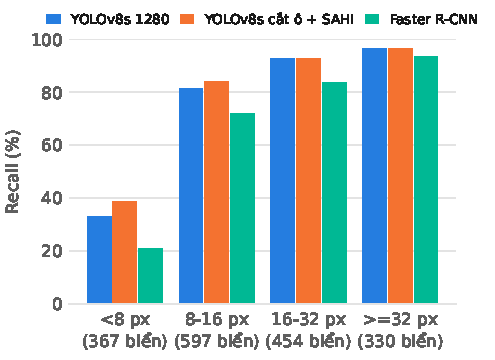
\includegraphics[width=\columnwidth]{figures/recall_theo_kich_thuoc.pdf}
\caption{Recall theo kích thước biển ($\sqrt{wh}$ trên ảnh gốc), tập test. Số dưới trục là số biển trong mỗi nhóm.}
\label{fig:recall-size}
\end{figure}

\subsection{Nhầm lớp tập trung ở ba lớp biển tròn viền đỏ}
\label{sec:confusion}

Ở YOLOv8s 1280, 30 trong 33 lần nhầm lớp (91\%) xảy ra giữa \textit{Cấm rẽ}, \textit{Giới hạn tốc độ} và \textit{Cấm còn lại}. Tỉ lệ bị gán sai lớp của ba lớp này lần lượt là 9,9\%, 11,4\% và 8,5\%, trong khi bốn lớp còn lại không quá 0,4\%.
Ba lớp này có cùng hình tròn, nền trắng, viền đỏ, chỉ khác hình vẽ ở giữa. Với biển 10 pixel, phần ở giữa chỉ còn vài pixel.
\textit{Cấm ngược chiều} là trường hợp ngược lại: lớp này có tới 90,5\% box nhỏ nhưng vẫn đạt AP50 84,7 trên test, vì nền đỏ đặc với vạch trắng ngang không giống lớp nào khác.
Vì vậy, độ khó của một lớp phụ thuộc vào việc nó có giống lớp khác không, hơn là vào kích thước biển.
Faster R-CNN nhầm nặng hơn hẳn: 28,4\% biển \textit{Cấm rẽ} bị gán sai lớp, chủ yếu thành \textit{Cấm còn lại}.

Nhóm xem lại bằng mắt cả 33 trường hợp nhầm lớp của YOLOv8s 1280:
\begin{itemize}
\item Ít nhất 7 trường hợp là \emph{nhãn sai, mô hình đúng}: biển ``50'' và ``80'' bị ghi \textit{Cấm còn lại}, biển hạn chế tải trọng ``10T'' bị ghi \textit{Giới hạn tốc độ}, biển tam giác cảnh báo bị ghi \textit{Hiệu lệnh}.
\item 4 trường hợp là lỗi rõ ràng của mô hình, ví dụ biển cấm rẽ rõ nét bị đoán thành \textit{Giới hạn tốc độ}.
\item Khoảng 19 trường hợp còn lại quá nhỏ hoặc quá mờ để người xem phân xử.
\end{itemize}

\subsection{Một phần ``báo nhầm nền'' là biển thiếu nhãn}
\label{sec:missing-labels}

Nhóm cũng xem lại 28 dự đoán bị tính là báo nhầm nền có độ tin cậy $\geq 0{,}6$, tức là các dự đoán không chồng lên box thật nào.
Ít nhất 15 trường hợp trúng một biển báo rõ ràng thuộc 7 lớp nhưng không được gán nhãn. Ví dụ: biển cấm đỗ và biển cấm rẽ trên cùng một cột, biển cảnh báo tam giác, biển ``10'' (Hình~\ref{fig:examples}, cột cuối).
Khoảng 5 trường hợp khác có thể cũng là biển. Chỉ khoảng 8 trường hợp là nền thật, chủ yếu là các mảng tối mờ.
Như vậy, nhãn test vừa thiếu biển vừa có nhãn sai lớp, và cả hai đều làm điểm của mô hình thấp hơn khả năng thật. Mức chênh này chưa được định lượng.

\begin{figure*}[t]
\centering
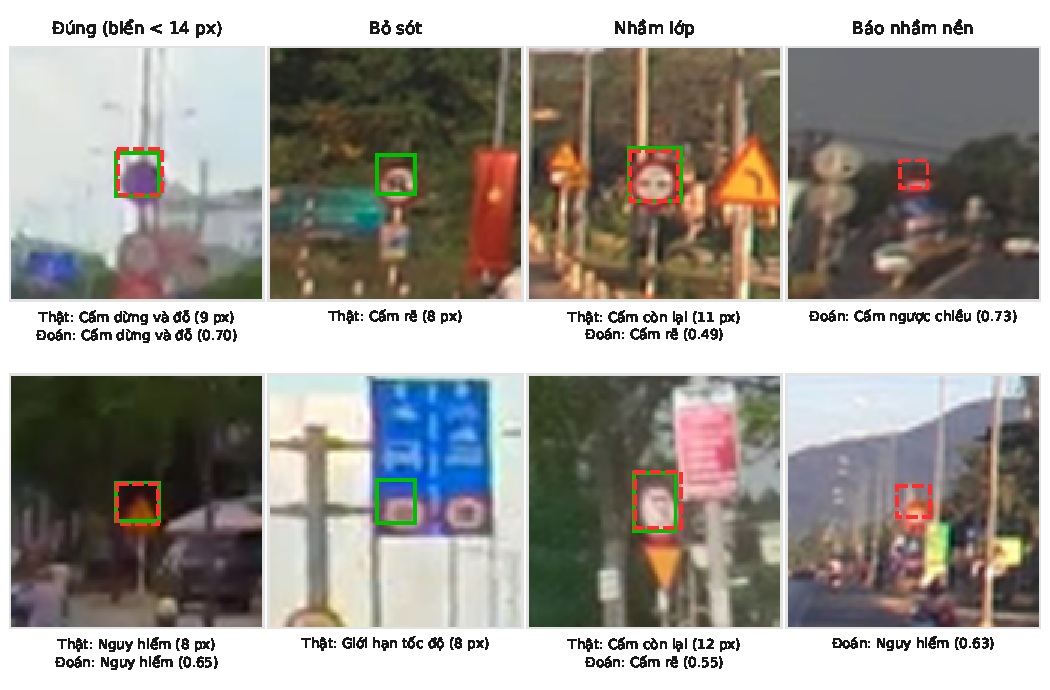
\includegraphics[width=0.92\textwidth]{figures/vi_du_du_doan.pdf}
\caption{Ví dụ dự đoán của YOLOv8s 1280 trên tập test (khung xanh liền: nhãn thật; khung đỏ đứt: dự đoán).
Cột 3, hàng dưới: biển có mũi tên rẽ bị gạch (\textit{Cấm rẽ}) nhưng bị gán nhãn \textit{Cấm còn lại}, nên dự đoán đúng của mô hình bị tính là nhầm lớp.
Cột 4: dự đoán không có nhãn thật tương ứng; hàng dưới trúng một biển thật không được gán nhãn.}
\label{fig:examples}
\end{figure*}

\subsection{Biển đứng cụm không bị bỏ sót nhiều hơn}
\label{sec:clusters}

43\% biển trong test đứng sát một biển khác (khe hở nhỏ hơn nửa cạnh của biển nhỏ hơn), thường là nhiều biển gắn trên cùng một cột.
Nếu chỉ nhìn số chung, biển trong cụm có vẻ bị bỏ sót nhiều hơn: recall 73,8\% so với 79,5\% với YOLOv8s 1280.
Nhưng biển trong cụm nhỏ hơn nhiều: 67,6\% dưới 16 pixel, so với 45,8\% ở biển đứng riêng.
Khi so trong từng nhóm kích thước, biển trong cụm được tìm thấy ngang bằng hoặc nhiều hơn (8--16 pixel: 86,0\% so với 77,7\%).
Vậy chênh lệch chung là do kích thước biển (biến gây nhiễu), không phải do NMS xóa nhầm biển đứng sát nhau. Ngưỡng NMS 0,65 theo từng lớp là đủ an toàn.

\subsection{Thí nghiệm: rò rỉ dữ liệu khi chia ngẫu nhiên}
\label{sec:leakage}

Để đo tác động của cách chia tập, nhóm lấy tập train (2.933 ảnh, 28 tuyến đường) chia lại thành train$'$/val$'$ (1.994/939 ảnh) theo hai cách: ngẫu nhiên theo ảnh, và theo tuyến đường.
Hai mô hình YOLOv8n (imgsz 1280, 50 epoch, cùng seed) được huấn luyện giống hệt nhau, chỉ khác cách chia.
Cả hai được chấm trên val$'$ của chính nó, và trên tập val gốc gồm 5 tuyến đường cả hai chưa từng thấy (Bảng~\ref{tab:leakage}). Tập test không được dùng trong thí nghiệm này.

\begin{table}[t]
\centering
\small
\begin{tabular}{lccc}
\toprule
Cách chia & val$'$ & Đường mới & Chênh \\
\midrule
Ngẫu nhiên    & \textbf{78,5} & \textbf{72,8} & $+5{,}7$ \\
Theo đường    & 62,9 & 69,9 & $-7{,}0$ \\
\bottomrule
\end{tabular}
\caption{mAP@0.5 (\%) của thí nghiệm rò rỉ. Với cách chia ngẫu nhiên, 88\% ảnh val$'$ có khung hình liền kề nằm trong train$'$.}
\label{tab:leakage}
\end{table}

Trên val$'$, mô hình chia ngẫu nhiên hơn mô hình chia theo đường 15,6 điểm. Trên cùng các tuyến đường mới, nó chỉ hơn 2,9 điểm.
Vậy phần lớn khoảng cách trên val$'$ là ảo: 88\% ảnh val$'$ có một khung hình gần như giống hệt trong train$'$.
Nếu tin vào val$'$ chia ngẫu nhiên, ta đánh giá khả năng trên đường mới cao hơn thực tế 5,7 điểm.
Phần hơn 2,9 điểm còn lại có thể vì mô hình chia ngẫu nhiên được thấy cả 28 tuyến đường, còn mô hình kia chỉ thấy 23.
Thí nghiệm cũng cho thấy hai bộ 5 tuyến đường có thể chênh nhau tới 7 điểm (62,9 so với 69,9). Điều này giúp giải thích vì sao kết quả trên val và test của nhóm lệch nhau 5--6 điểm.

\subsection{Thí nghiệm: xử lý mất cân bằng lớp}
\label{sec:imbalance}

Mục~\ref{sec:confusion} cho thấy các lớp ít mẫu (\textit{Cấm rẽ}, \textit{Giới hạn tốc độ}) cũng là các lớp hay bị nhầm. Nhóm thử hai cách cân bằng lớp trên cấu hình YOLOv8s 1280, mỗi cách chỉ thay đổi đúng một yếu tố:
\begin{itemize}
\item \textbf{Repeat Factor Sampling} (RFS) \citep{gupta2019lvis}: lặp lại các ảnh chứa lớp hiếm với hệ số $r_c = \max(1, \sqrt{t/f_c})$, trong đó $f_c$ là tỉ lệ ảnh có lớp $c$ và $t = 0{,}3$. Cách này giảm tỉ lệ số box lớp nhiều nhất / ít nhất từ 4,4 xuống 2,9.
\item \textbf{Trọng số lớp} trong loss phân loại, tỉ lệ với $(1/n_c)^{0{,}5}$, trong đó $n_c$ là số box của lớp $c$ (tham số \texttt{cls\_pw} của Ultralytics).
\end{itemize}

\begin{table}[t]
\centering
\small
\begin{tabular}{lccc}
\toprule
& Gốc & RFS & Trọng số lớp \\
\midrule
mAP@0.5          & \textbf{82,2} & 81,0 & 81,1 \\
AP50 Cấm rẽ          & \textbf{75,0} & 71,4 & 74,9 \\
AP50 Giới hạn tốc độ & \textbf{77,7} & 73,1 & 71,6$^{*}$ \\
AP50 Hiệu lệnh       & 78,6 & \textbf{80,7} & 78,7 \\
Nhầm trong nhóm tròn đỏ & \textbf{47} & 56 & 50 \\
\bottomrule
\end{tabular}
\caption{Thí nghiệm mất cân bằng lớp trên val (\%). Dòng cuối là số biển bị nhầm giữa ba lớp tròn viền đỏ. $^{*}$: chênh lệch so với gốc có ý nghĩa thống kê (bootstrap, khoảng tin cậy 95\% là $[-10{,}2; -1{,}6]$). Mọi chênh lệch khác đều nằm trong khoảng dao động.}
\label{tab:imbalance}
\end{table}

Cả hai cách đều \emph{không} cải thiện các lớp hiếm (Bảng~\ref{tab:imbalance}). Có bốn nguyên nhân:
\begin{enumerate}
\item \textbf{Lỗi chỉ bị chuyển chỗ, không mất đi.} Tổng số lần nhầm trong nhóm tròn đỏ không giảm (47 tăng lên 56 và 50).
  Với trọng số lớp, \textit{Cấm rẽ} được nhận đúng thêm 3 biển, nhưng số dự đoán \textit{Cấm rẽ} sai tăng từ 9 lên 17. \textit{Giới hạn tốc độ} bị kéo sang \textit{Cấm rẽ} nhiều hơn, nên AP của nó giảm 6,1 điểm.
  Trọng số chỉ dịch ranh giới quyết định giữa các lớp trông giống nhau, chứ không giúp phân biệt chúng tốt hơn.
\item \textbf{Lặp ảnh thì lặp luôn lớp gây nhầm.} 49\% ảnh có \textit{Giới hạn tốc độ} cũng có \textit{Cấm còn lại}, trong khi tỉ lệ chung chỉ 25\%. Vì vậy RFS lặp chính lớp mà \textit{Giới hạn tốc độ} hay bị nhầm sang.
\item \textbf{Nhầm lớp không phải lỗi chính.} Chỉ 3,2\% biển bị nhầm lớp, trong khi 16,7\% bị bỏ sót (Mục~\ref{sec:small}). Cân bằng lớp không làm recall biển nhỏ tăng.
\item \textbf{Mức mất cân bằng vừa phải} (4,4 lần). RFS được thiết kế cho dữ liệu đuôi dài, nơi lớp hiếm ít hơn hàng trăm lần.
\end{enumerate}
Không thấy dấu hiệu học thuộc do lặp ảnh: loss phân loại trên val vẫn giảm tới epoch cuối.
Với nhầm lẫn giữa các lớp tròn viền đỏ, cách hợp lý hơn là cho mô hình nhìn rõ phần giữa biển (độ phân giải cao hơn, hoặc phân loại lại vùng cắt quanh biển) và sửa nhãn sai (Mục~\ref{sec:confusion}).

% Cần: booktabs, graphicx; hình trong figures/ (tạo bằng evaluation/make_report_figures.py)
% Số liệu: reports/errors/*_test, experiments/leakage, experiments/imbalance
% ------------------------------------------------

\section{Phân tích}
\label{sec:analysis}

Mục này dùng các mô hình cuối trên tập test (1.748 biển) để tách lỗi thành ba loại, theo cách ghép dự đoán với nhãn ở IoU $\geq 0{,}5$:
\begin{itemize}
\item \emph{bỏ sót}: không có dự đoán nào trùng biển;
\item \emph{nhầm lớp}: dự đoán trùng biển nhưng sai lớp;
\item \emph{báo nhầm nền}: dự đoán không trùng biển nào.
\end{itemize}
Ngưỡng độ tin cậy của mỗi mô hình được chọn sao cho F1 cao nhất, vì thang điểm tin cậy của YOLO và Faster R-CNN khác nhau. Phân tích trên tập val cho cùng các kết luận.

\subsection{Lỗi chính là bỏ sót biển nhỏ}
\label{sec:small}

Với YOLOv8s 1280, 77,1\% biển được tìm đúng, 21,1\% bị bỏ sót, và chỉ 1,9\% bị nhận sai lớp.
Trong 368 biển bị bỏ sót, 337 biển (92\%) nhỏ hơn 16 pixel. Hai mô hình còn lại cũng như vậy: 91\% với cắt ô + SAHI và 87\% với Faster R-CNN.
Hình~\ref{fig:recall-size} cho thấy với YOLO, recall gần như bão hòa ($> 92\%$) ở biển từ 16 pixel trở lên. Recall giảm ở biển 8--16 pixel, và ở biển dưới 8 pixel chỉ còn 21--39\% với cả ba mô hình.
Ở imgsz 1280, một biển 8 pixel trên ảnh gốc chỉ còn khoảng 6 pixel, nhỏ hơn một ô của bản đồ đặc trưng mịn nhất của YOLOv8 (stride 8). Cắt ô giữ nguyên độ phân giải gốc, nên tăng recall ở nhóm này từ 33,0\% lên 38,7\%.

Faster R-CNN kém YOLO ở mọi nhóm kích thước, kể cả nhóm $\geq 32$ pixel (93,6\% so với 96,4\%). Ảnh đưa vào Faster R-CNN còn lớn hơn (cạnh dài 1800 pixel), nên khoảng cách này không đến từ độ phân giải. Nhiều khả năng nó đến từ thiết lập huấn luyện: 30 epoch, augmentation đơn giản, so với 50 epoch có mosaic của YOLO. Faster R-CNN cũng báo nhầm nền nhiều hơn (156 so với 97 box).

\begin{figure}[t]
\centering
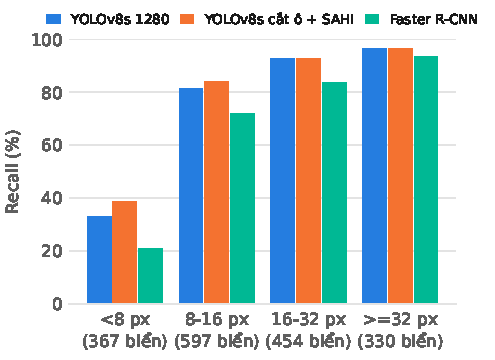
\includegraphics[width=\columnwidth]{figures/recall_theo_kich_thuoc.pdf}
\caption{Recall theo kích thước biển ($\sqrt{wh}$ trên ảnh gốc), tập test. Số dưới trục là số biển trong mỗi nhóm.}
\label{fig:recall-size}
\end{figure}

\subsection{Nhầm lớp tập trung ở ba lớp biển tròn viền đỏ}
\label{sec:confusion}

Ở YOLOv8s 1280, 30 trong 33 lần nhầm lớp (91\%) xảy ra giữa \textit{Cấm rẽ}, \textit{Giới hạn tốc độ} và \textit{Cấm còn lại}. Tỉ lệ bị gán sai lớp của ba lớp này lần lượt là 9,9\%, 11,4\% và 8,5\%, trong khi bốn lớp còn lại không quá 0,4\%.
Ba lớp này có cùng hình tròn, nền trắng, viền đỏ, chỉ khác hình vẽ ở giữa. Với biển 10 pixel, phần ở giữa chỉ còn vài pixel.
\textit{Cấm ngược chiều} là trường hợp ngược lại: lớp này có tới 90,5\% box nhỏ nhưng vẫn đạt AP50 84,7 trên test, vì nền đỏ đặc với vạch trắng ngang không giống lớp nào khác.
Vì vậy, độ khó của một lớp phụ thuộc vào việc nó có giống lớp khác không, hơn là vào kích thước biển.
Faster R-CNN nhầm nặng hơn hẳn: 28,4\% biển \textit{Cấm rẽ} bị gán sai lớp, chủ yếu thành \textit{Cấm còn lại}.

Nhóm xem lại bằng mắt cả 33 trường hợp nhầm lớp của YOLOv8s 1280:
\begin{itemize}
\item Ít nhất 7 trường hợp là \emph{nhãn sai, mô hình đúng}: biển ``50'' và ``80'' bị ghi \textit{Cấm còn lại}, biển hạn chế tải trọng ``10T'' bị ghi \textit{Giới hạn tốc độ}, biển tam giác cảnh báo bị ghi \textit{Hiệu lệnh}.
\item 4 trường hợp là lỗi rõ ràng của mô hình, ví dụ biển cấm rẽ rõ nét bị đoán thành \textit{Giới hạn tốc độ}.
\item Khoảng 19 trường hợp còn lại quá nhỏ hoặc quá mờ để người xem phân xử.
\end{itemize}

\subsection{Một phần ``báo nhầm nền'' là biển thiếu nhãn}
\label{sec:missing-labels}

Nhóm cũng xem lại 28 dự đoán bị tính là báo nhầm nền có độ tin cậy $\geq 0{,}6$, tức là các dự đoán không chồng lên box thật nào.
Ít nhất 15 trường hợp trúng một biển báo rõ ràng thuộc 7 lớp nhưng không được gán nhãn. Ví dụ: biển cấm đỗ và biển cấm rẽ trên cùng một cột, biển cảnh báo tam giác, biển ``10'' (Hình~\ref{fig:examples}, cột cuối).
Khoảng 5 trường hợp khác có thể cũng là biển. Chỉ khoảng 8 trường hợp là nền thật, chủ yếu là các mảng tối mờ.
Như vậy, nhãn test vừa thiếu biển vừa có nhãn sai lớp, và cả hai đều làm điểm của mô hình thấp hơn khả năng thật. Mức chênh này chưa được định lượng.

\begin{figure*}[t]
\centering
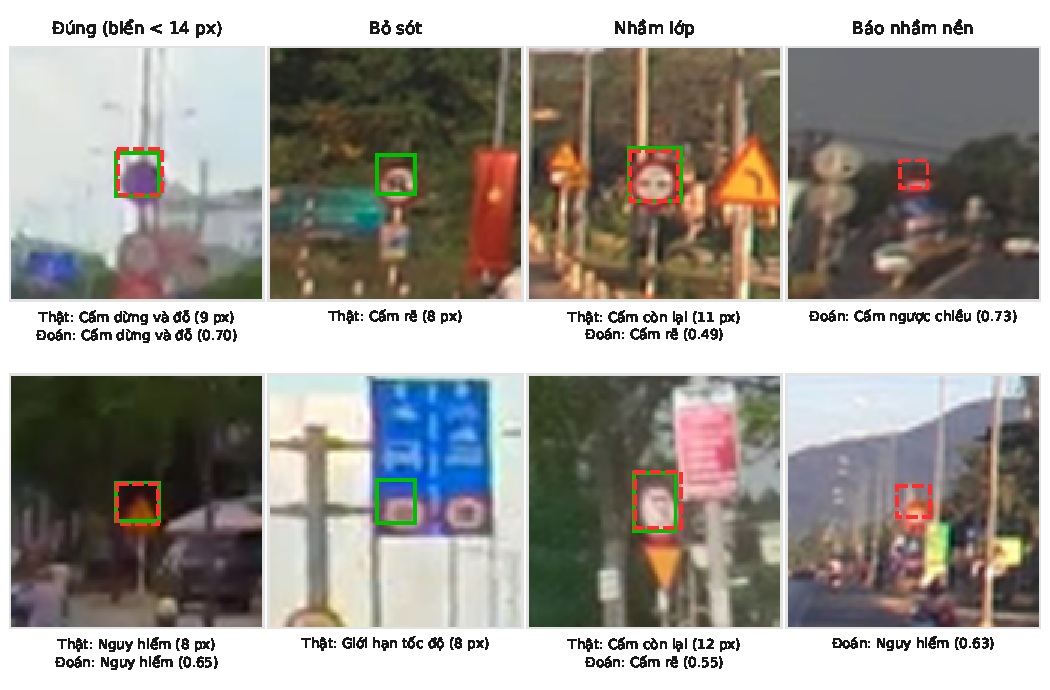
\includegraphics[width=0.92\textwidth]{figures/vi_du_du_doan.pdf}
\caption{Ví dụ dự đoán của YOLOv8s 1280 trên tập test (khung xanh liền: nhãn thật; khung đỏ đứt: dự đoán).
Cột 3, hàng dưới: biển có mũi tên rẽ bị gạch (\textit{Cấm rẽ}) nhưng bị gán nhãn \textit{Cấm còn lại}, nên dự đoán đúng của mô hình bị tính là nhầm lớp.
Cột 4: dự đoán không có nhãn thật tương ứng; hàng dưới trúng một biển thật không được gán nhãn.}
\label{fig:examples}
\end{figure*}

\subsection{Biển đứng cụm không bị bỏ sót nhiều hơn}
\label{sec:clusters}

43\% biển trong test đứng sát một biển khác (khe hở nhỏ hơn nửa cạnh của biển nhỏ hơn), thường là nhiều biển gắn trên cùng một cột.
Nếu chỉ nhìn số chung, biển trong cụm có vẻ bị bỏ sót nhiều hơn: recall 73,8\% so với 79,5\% với YOLOv8s 1280.
Nhưng biển trong cụm nhỏ hơn nhiều: 67,6\% dưới 16 pixel, so với 45,8\% ở biển đứng riêng.
Khi so trong từng nhóm kích thước, biển trong cụm được tìm thấy ngang bằng hoặc nhiều hơn (8--16 pixel: 86,0\% so với 77,7\%).
Vậy chênh lệch chung là do kích thước biển (biến gây nhiễu), không phải do NMS xóa nhầm biển đứng sát nhau. Ngưỡng NMS 0,65 theo từng lớp là đủ an toàn.

\subsection{Thí nghiệm: rò rỉ dữ liệu khi chia ngẫu nhiên}
\label{sec:leakage}

Để đo tác động của cách chia tập, nhóm lấy tập train (2.933 ảnh, 28 tuyến đường) chia lại thành train$'$/val$'$ (1.994/939 ảnh) theo hai cách: ngẫu nhiên theo ảnh, và theo tuyến đường.
Hai mô hình YOLOv8n (imgsz 1280, 50 epoch, cùng seed) được huấn luyện giống hệt nhau, chỉ khác cách chia.
Cả hai được chấm trên val$'$ của chính nó, và trên tập val gốc gồm 5 tuyến đường cả hai chưa từng thấy (Bảng~\ref{tab:leakage}). Tập test không được dùng trong thí nghiệm này.

\begin{table}[t]
\centering
\small
\begin{tabular}{lccc}
\toprule
Cách chia & val$'$ & Đường mới & Chênh \\
\midrule
Ngẫu nhiên    & \textbf{78,5} & \textbf{72,8} & $+5{,}7$ \\
Theo đường    & 62,9 & 69,9 & $-7{,}0$ \\
\bottomrule
\end{tabular}
\caption{mAP@0.5 (\%) của thí nghiệm rò rỉ. Với cách chia ngẫu nhiên, 88\% ảnh val$'$ có khung hình liền kề nằm trong train$'$.}
\label{tab:leakage}
\end{table}

Trên val$'$, mô hình chia ngẫu nhiên hơn mô hình chia theo đường 15,6 điểm. Trên cùng các tuyến đường mới, nó chỉ hơn 2,9 điểm.
Vậy phần lớn khoảng cách trên val$'$ là ảo: 88\% ảnh val$'$ có một khung hình gần như giống hệt trong train$'$.
Nếu tin vào val$'$ chia ngẫu nhiên, ta đánh giá khả năng trên đường mới cao hơn thực tế 5,7 điểm.
Phần hơn 2,9 điểm còn lại có thể vì mô hình chia ngẫu nhiên được thấy cả 28 tuyến đường, còn mô hình kia chỉ thấy 23.
Thí nghiệm cũng cho thấy hai bộ 5 tuyến đường có thể chênh nhau tới 7 điểm (62,9 so với 69,9). Điều này giúp giải thích vì sao kết quả trên val và test của nhóm lệch nhau 5--6 điểm.

\subsection{Thí nghiệm: xử lý mất cân bằng lớp}
\label{sec:imbalance}

Mục~\ref{sec:confusion} cho thấy các lớp ít mẫu (\textit{Cấm rẽ}, \textit{Giới hạn tốc độ}) cũng là các lớp hay bị nhầm. Nhóm thử hai cách cân bằng lớp trên cấu hình YOLOv8s 1280, mỗi cách chỉ thay đổi đúng một yếu tố:
\begin{itemize}
\item \textbf{Repeat Factor Sampling} (RFS) \citep{gupta2019lvis}: lặp lại các ảnh chứa lớp hiếm với hệ số $r_c = \max(1, \sqrt{t/f_c})$, trong đó $f_c$ là tỉ lệ ảnh có lớp $c$ và $t = 0{,}3$. Cách này giảm tỉ lệ số box lớp nhiều nhất / ít nhất từ 4,4 xuống 2,9.
\item \textbf{Trọng số lớp} trong loss phân loại, tỉ lệ với $(1/n_c)^{0{,}5}$, trong đó $n_c$ là số box của lớp $c$ (tham số \texttt{cls\_pw} của Ultralytics).
\end{itemize}

\begin{table}[t]
\centering
\small
\begin{tabular}{lccc}
\toprule
& Gốc & RFS & Trọng số lớp \\
\midrule
mAP@0.5          & \textbf{82,2} & 81,0 & 81,1 \\
AP50 Cấm rẽ          & \textbf{75,0} & 71,4 & 74,9 \\
AP50 Giới hạn tốc độ & \textbf{77,7} & 73,1 & 71,6$^{*}$ \\
AP50 Hiệu lệnh       & 78,6 & \textbf{80,7} & 78,7 \\
Nhầm trong nhóm tròn đỏ & \textbf{47} & 56 & 50 \\
\bottomrule
\end{tabular}
\caption{Thí nghiệm mất cân bằng lớp trên val (\%). Dòng cuối là số biển bị nhầm giữa ba lớp tròn viền đỏ. $^{*}$: chênh lệch so với gốc có ý nghĩa thống kê (bootstrap, khoảng tin cậy 95\% là $[-10{,}2; -1{,}6]$). Mọi chênh lệch khác đều nằm trong khoảng dao động.}
\label{tab:imbalance}
\end{table}

Cả hai cách đều \emph{không} cải thiện các lớp hiếm (Bảng~\ref{tab:imbalance}). Có bốn nguyên nhân:
\begin{enumerate}
\item \textbf{Lỗi chỉ bị chuyển chỗ, không mất đi.} Tổng số lần nhầm trong nhóm tròn đỏ không giảm (47 tăng lên 56 và 50).
  Với trọng số lớp, \textit{Cấm rẽ} được nhận đúng thêm 3 biển, nhưng số dự đoán \textit{Cấm rẽ} sai tăng từ 9 lên 17. \textit{Giới hạn tốc độ} bị kéo sang \textit{Cấm rẽ} nhiều hơn, nên AP của nó giảm 6,1 điểm.
  Trọng số chỉ dịch ranh giới quyết định giữa các lớp trông giống nhau, chứ không giúp phân biệt chúng tốt hơn.
\item \textbf{Lặp ảnh thì lặp luôn lớp gây nhầm.} 49\% ảnh có \textit{Giới hạn tốc độ} cũng có \textit{Cấm còn lại}, trong khi tỉ lệ chung chỉ 25\%. Vì vậy RFS lặp chính lớp mà \textit{Giới hạn tốc độ} hay bị nhầm sang.
\item \textbf{Nhầm lớp không phải lỗi chính.} Chỉ 3,2\% biển bị nhầm lớp, trong khi 16,7\% bị bỏ sót (Mục~\ref{sec:small}). Cân bằng lớp không làm recall biển nhỏ tăng.
\item \textbf{Mức mất cân bằng vừa phải} (4,4 lần). RFS được thiết kế cho dữ liệu đuôi dài, nơi lớp hiếm ít hơn hàng trăm lần.
\end{enumerate}
Không thấy dấu hiệu học thuộc do lặp ảnh: loss phân loại trên val vẫn giảm tới epoch cuối.
Với nhầm lẫn giữa các lớp tròn viền đỏ, cách hợp lý hơn là cho mô hình nhìn rõ phần giữa biển (độ phân giải cao hơn, hoặc phân loại lại vùng cắt quanh biển) và sửa nhãn sai (Mục~\ref{sec:confusion}).

% Cần: booktabs, graphicx; hình trong figures/ (tạo bằng evaluation/make_report_figures.py)
% Số liệu: reports/errors/*_test, experiments/leakage, experiments/imbalance
% ------------------------------------------------

\section{Phân tích}
\label{sec:analysis}

Mục này dùng các mô hình cuối trên tập test (1.748 biển) để tách lỗi thành ba loại, theo cách ghép dự đoán với nhãn ở IoU $\geq 0{,}5$:
\begin{itemize}
\item \emph{bỏ sót}: không có dự đoán nào trùng biển;
\item \emph{nhầm lớp}: dự đoán trùng biển nhưng sai lớp;
\item \emph{báo nhầm nền}: dự đoán không trùng biển nào.
\end{itemize}
Ngưỡng độ tin cậy của mỗi mô hình được chọn sao cho F1 cao nhất, vì thang điểm tin cậy của YOLO và Faster R-CNN khác nhau. Phân tích trên tập val cho cùng các kết luận.

\subsection{Lỗi chính là bỏ sót biển nhỏ}
\label{sec:small}

Với YOLOv8s 1280, 77,1\% biển được tìm đúng, 21,1\% bị bỏ sót, và chỉ 1,9\% bị nhận sai lớp.
Trong 368 biển bị bỏ sót, 337 biển (92\%) nhỏ hơn 16 pixel. Hai mô hình còn lại cũng như vậy: 91\% với cắt ô + SAHI và 87\% với Faster R-CNN.
Hình~\ref{fig:recall-size} cho thấy với YOLO, recall gần như bão hòa ($> 92\%$) ở biển từ 16 pixel trở lên. Recall giảm ở biển 8--16 pixel, và ở biển dưới 8 pixel chỉ còn 21--39\% với cả ba mô hình.
Ở imgsz 1280, một biển 8 pixel trên ảnh gốc chỉ còn khoảng 6 pixel, nhỏ hơn một ô của bản đồ đặc trưng mịn nhất của YOLOv8 (stride 8). Cắt ô giữ nguyên độ phân giải gốc, nên tăng recall ở nhóm này từ 33,0\% lên 38,7\%.

Faster R-CNN kém YOLO ở mọi nhóm kích thước, kể cả nhóm $\geq 32$ pixel (93,6\% so với 96,4\%). Ảnh đưa vào Faster R-CNN còn lớn hơn (cạnh dài 1800 pixel), nên khoảng cách này không đến từ độ phân giải. Nhiều khả năng nó đến từ thiết lập huấn luyện: 30 epoch, augmentation đơn giản, so với 50 epoch có mosaic của YOLO. Faster R-CNN cũng báo nhầm nền nhiều hơn (156 so với 97 box).

\begin{figure}[t]
\centering
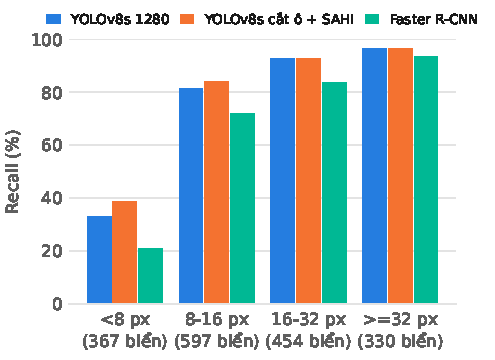
\includegraphics[width=\columnwidth]{figures/recall_theo_kich_thuoc.pdf}
\caption{Recall theo kích thước biển ($\sqrt{wh}$ trên ảnh gốc), tập test. Số dưới trục là số biển trong mỗi nhóm.}
\label{fig:recall-size}
\end{figure}

\subsection{Nhầm lớp tập trung ở ba lớp biển tròn viền đỏ}
\label{sec:confusion}

Ở YOLOv8s 1280, 30 trong 33 lần nhầm lớp (91\%) xảy ra giữa \textit{Cấm rẽ}, \textit{Giới hạn tốc độ} và \textit{Cấm còn lại}. Tỉ lệ bị gán sai lớp của ba lớp này lần lượt là 9,9\%, 11,4\% và 8,5\%, trong khi bốn lớp còn lại không quá 0,4\%.
Ba lớp này có cùng hình tròn, nền trắng, viền đỏ, chỉ khác hình vẽ ở giữa. Với biển 10 pixel, phần ở giữa chỉ còn vài pixel.
\textit{Cấm ngược chiều} là trường hợp ngược lại: lớp này có tới 90,5\% box nhỏ nhưng vẫn đạt AP50 84,7 trên test, vì nền đỏ đặc với vạch trắng ngang không giống lớp nào khác.
Vì vậy, độ khó của một lớp phụ thuộc vào việc nó có giống lớp khác không, hơn là vào kích thước biển.
Faster R-CNN nhầm nặng hơn hẳn: 28,4\% biển \textit{Cấm rẽ} bị gán sai lớp, chủ yếu thành \textit{Cấm còn lại}.

Nhóm xem lại bằng mắt cả 33 trường hợp nhầm lớp của YOLOv8s 1280:
\begin{itemize}
\item Ít nhất 7 trường hợp là \emph{nhãn sai, mô hình đúng}: biển ``50'' và ``80'' bị ghi \textit{Cấm còn lại}, biển hạn chế tải trọng ``10T'' bị ghi \textit{Giới hạn tốc độ}, biển tam giác cảnh báo bị ghi \textit{Hiệu lệnh}.
\item 4 trường hợp là lỗi rõ ràng của mô hình, ví dụ biển cấm rẽ rõ nét bị đoán thành \textit{Giới hạn tốc độ}.
\item Khoảng 19 trường hợp còn lại quá nhỏ hoặc quá mờ để người xem phân xử.
\end{itemize}

\subsection{Một phần ``báo nhầm nền'' là biển thiếu nhãn}
\label{sec:missing-labels}

Nhóm cũng xem lại 28 dự đoán bị tính là báo nhầm nền có độ tin cậy $\geq 0{,}6$, tức là các dự đoán không chồng lên box thật nào.
Ít nhất 15 trường hợp trúng một biển báo rõ ràng thuộc 7 lớp nhưng không được gán nhãn. Ví dụ: biển cấm đỗ và biển cấm rẽ trên cùng một cột, biển cảnh báo tam giác, biển ``10'' (Hình~\ref{fig:examples}, cột cuối).
Khoảng 5 trường hợp khác có thể cũng là biển. Chỉ khoảng 8 trường hợp là nền thật, chủ yếu là các mảng tối mờ.
Như vậy, nhãn test vừa thiếu biển vừa có nhãn sai lớp, và cả hai đều làm điểm của mô hình thấp hơn khả năng thật. Mức chênh này chưa được định lượng.

\begin{figure*}[t]
\centering
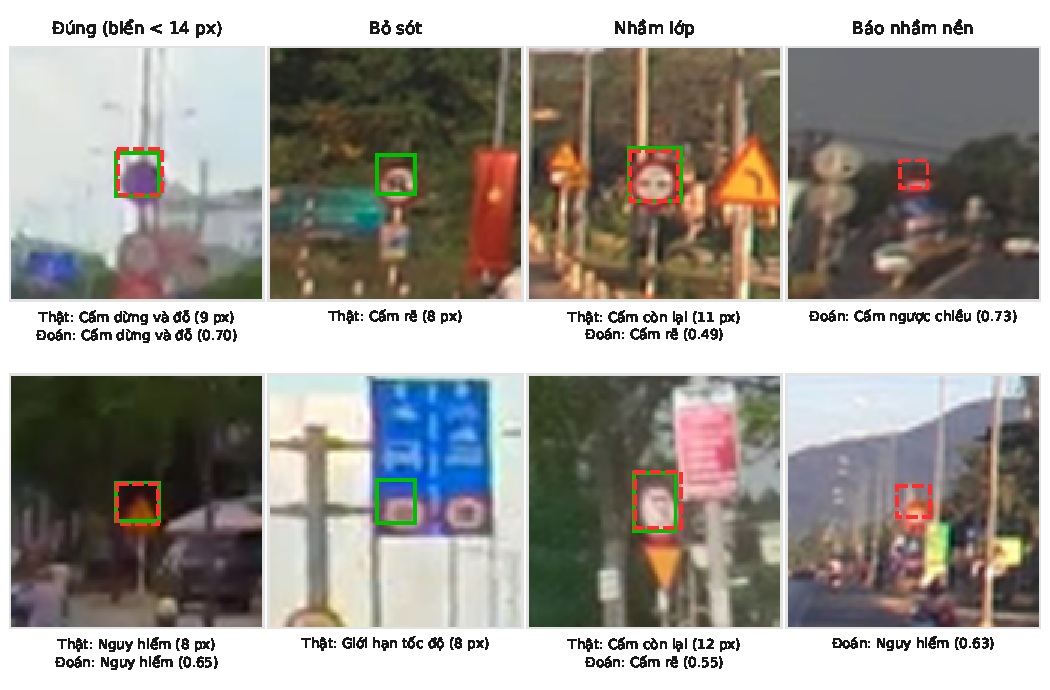
\includegraphics[width=0.92\textwidth]{figures/vi_du_du_doan.pdf}
\caption{Ví dụ dự đoán của YOLOv8s 1280 trên tập test (khung xanh liền: nhãn thật; khung đỏ đứt: dự đoán).
Cột 3, hàng dưới: biển có mũi tên rẽ bị gạch (\textit{Cấm rẽ}) nhưng bị gán nhãn \textit{Cấm còn lại}, nên dự đoán đúng của mô hình bị tính là nhầm lớp.
Cột 4: dự đoán không có nhãn thật tương ứng; hàng dưới trúng một biển thật không được gán nhãn.}
\label{fig:examples}
\end{figure*}

\subsection{Biển đứng cụm không bị bỏ sót nhiều hơn}
\label{sec:clusters}

43\% biển trong test đứng sát một biển khác (khe hở nhỏ hơn nửa cạnh của biển nhỏ hơn), thường là nhiều biển gắn trên cùng một cột.
Nếu chỉ nhìn số chung, biển trong cụm có vẻ bị bỏ sót nhiều hơn: recall 73,8\% so với 79,5\% với YOLOv8s 1280.
Nhưng biển trong cụm nhỏ hơn nhiều: 67,6\% dưới 16 pixel, so với 45,8\% ở biển đứng riêng.
Khi so trong từng nhóm kích thước, biển trong cụm được tìm thấy ngang bằng hoặc nhiều hơn (8--16 pixel: 86,0\% so với 77,7\%).
Vậy chênh lệch chung là do kích thước biển (biến gây nhiễu), không phải do NMS xóa nhầm biển đứng sát nhau. Ngưỡng NMS 0,65 theo từng lớp là đủ an toàn.

\subsection{Thí nghiệm: rò rỉ dữ liệu khi chia ngẫu nhiên}
\label{sec:leakage}

Để đo tác động của cách chia tập, nhóm lấy tập train (2.933 ảnh, 28 tuyến đường) chia lại thành train$'$/val$'$ (1.994/939 ảnh) theo hai cách: ngẫu nhiên theo ảnh, và theo tuyến đường.
Hai mô hình YOLOv8n (imgsz 1280, 50 epoch, cùng seed) được huấn luyện giống hệt nhau, chỉ khác cách chia.
Cả hai được chấm trên val$'$ của chính nó, và trên tập val gốc gồm 5 tuyến đường cả hai chưa từng thấy (Bảng~\ref{tab:leakage}). Tập test không được dùng trong thí nghiệm này.

\begin{table}[t]
\centering
\small
\begin{tabular}{lccc}
\toprule
Cách chia & val$'$ & Đường mới & Chênh \\
\midrule
Ngẫu nhiên    & \textbf{78,5} & \textbf{72,8} & $+5{,}7$ \\
Theo đường    & 62,9 & 69,9 & $-7{,}0$ \\
\bottomrule
\end{tabular}
\caption{mAP@0.5 (\%) của thí nghiệm rò rỉ. Với cách chia ngẫu nhiên, 88\% ảnh val$'$ có khung hình liền kề nằm trong train$'$.}
\label{tab:leakage}
\end{table}

Trên val$'$, mô hình chia ngẫu nhiên hơn mô hình chia theo đường 15,6 điểm. Trên cùng các tuyến đường mới, nó chỉ hơn 2,9 điểm.
Vậy phần lớn khoảng cách trên val$'$ là ảo: 88\% ảnh val$'$ có một khung hình gần như giống hệt trong train$'$.
Nếu tin vào val$'$ chia ngẫu nhiên, ta đánh giá khả năng trên đường mới cao hơn thực tế 5,7 điểm.
Phần hơn 2,9 điểm còn lại có thể vì mô hình chia ngẫu nhiên được thấy cả 28 tuyến đường, còn mô hình kia chỉ thấy 23.
Thí nghiệm cũng cho thấy hai bộ 5 tuyến đường có thể chênh nhau tới 7 điểm (62,9 so với 69,9). Điều này giúp giải thích vì sao kết quả trên val và test của nhóm lệch nhau 5--6 điểm.

\subsection{Thí nghiệm: xử lý mất cân bằng lớp}
\label{sec:imbalance}

Mục~\ref{sec:confusion} cho thấy các lớp ít mẫu (\textit{Cấm rẽ}, \textit{Giới hạn tốc độ}) cũng là các lớp hay bị nhầm. Nhóm thử hai cách cân bằng lớp trên cấu hình YOLOv8s 1280, mỗi cách chỉ thay đổi đúng một yếu tố:
\begin{itemize}
\item \textbf{Repeat Factor Sampling} (RFS) \citep{gupta2019lvis}: lặp lại các ảnh chứa lớp hiếm với hệ số $r_c = \max(1, \sqrt{t/f_c})$, trong đó $f_c$ là tỉ lệ ảnh có lớp $c$ và $t = 0{,}3$. Cách này giảm tỉ lệ số box lớp nhiều nhất / ít nhất từ 4,4 xuống 2,9.
\item \textbf{Trọng số lớp} trong loss phân loại, tỉ lệ với $(1/n_c)^{0{,}5}$, trong đó $n_c$ là số box của lớp $c$ (tham số \texttt{cls\_pw} của Ultralytics).
\end{itemize}

\begin{table}[t]
\centering
\small
\begin{tabular}{lccc}
\toprule
& Gốc & RFS & Trọng số lớp \\
\midrule
mAP@0.5          & \textbf{82,2} & 81,0 & 81,1 \\
AP50 Cấm rẽ          & \textbf{75,0} & 71,4 & 74,9 \\
AP50 Giới hạn tốc độ & \textbf{77,7} & 73,1 & 71,6$^{*}$ \\
AP50 Hiệu lệnh       & 78,6 & \textbf{80,7} & 78,7 \\
Nhầm trong nhóm tròn đỏ & \textbf{47} & 56 & 50 \\
\bottomrule
\end{tabular}
\caption{Thí nghiệm mất cân bằng lớp trên val (\%). Dòng cuối là số biển bị nhầm giữa ba lớp tròn viền đỏ. $^{*}$: chênh lệch so với gốc có ý nghĩa thống kê (bootstrap, khoảng tin cậy 95\% là $[-10{,}2; -1{,}6]$). Mọi chênh lệch khác đều nằm trong khoảng dao động.}
\label{tab:imbalance}
\end{table}

Cả hai cách đều \emph{không} cải thiện các lớp hiếm (Bảng~\ref{tab:imbalance}). Có bốn nguyên nhân:
\begin{enumerate}
\item \textbf{Lỗi chỉ bị chuyển chỗ, không mất đi.} Tổng số lần nhầm trong nhóm tròn đỏ không giảm (47 tăng lên 56 và 50).
  Với trọng số lớp, \textit{Cấm rẽ} được nhận đúng thêm 3 biển, nhưng số dự đoán \textit{Cấm rẽ} sai tăng từ 9 lên 17. \textit{Giới hạn tốc độ} bị kéo sang \textit{Cấm rẽ} nhiều hơn, nên AP của nó giảm 6,1 điểm.
  Trọng số chỉ dịch ranh giới quyết định giữa các lớp trông giống nhau, chứ không giúp phân biệt chúng tốt hơn.
\item \textbf{Lặp ảnh thì lặp luôn lớp gây nhầm.} 49\% ảnh có \textit{Giới hạn tốc độ} cũng có \textit{Cấm còn lại}, trong khi tỉ lệ chung chỉ 25\%. Vì vậy RFS lặp chính lớp mà \textit{Giới hạn tốc độ} hay bị nhầm sang.
\item \textbf{Nhầm lớp không phải lỗi chính.} Chỉ 3,2\% biển bị nhầm lớp, trong khi 16,7\% bị bỏ sót (Mục~\ref{sec:small}). Cân bằng lớp không làm recall biển nhỏ tăng.
\item \textbf{Mức mất cân bằng vừa phải} (4,4 lần). RFS được thiết kế cho dữ liệu đuôi dài, nơi lớp hiếm ít hơn hàng trăm lần.
\end{enumerate}
Không thấy dấu hiệu học thuộc do lặp ảnh: loss phân loại trên val vẫn giảm tới epoch cuối.
Với nhầm lẫn giữa các lớp tròn viền đỏ, cách hợp lý hơn là cho mô hình nhìn rõ phần giữa biển (độ phân giải cao hơn, hoặc phân loại lại vùng cắt quanh biển) và sửa nhãn sai (Mục~\ref{sec:confusion}).

% ------------------------------------------------
% TỐC ĐỘ VÀ SUY LUẬN THỜI GIAN THỰC (phần của C). Ghép vào báo cáo chính bằng % ------------------------------------------------
% TỐC ĐỘ VÀ SUY LUẬN THỜI GIAN THỰC (phần của C). Ghép vào báo cáo chính bằng % ------------------------------------------------
% TỐC ĐỘ VÀ SUY LUẬN THỜI GIAN THỰC (phần của C). Ghép vào báo cáo chính bằng \input{sections/realtime}
% Số liệu: reports/latency_fps/summary.json (YOLO), summary1.json (Faster R-CNN)
% ------------------------------------------------

\section{Tốc độ và suy luận thời gian thực}
\label{sec:realtime}

Để đánh giá khả năng triển khai, nhóm xây dựng một pipeline xử lý video (thư mục \texttt{streaming/}). Pipeline đọc từng khung hình, phát hiện biển, theo dõi biển qua các khung hình bằng một bộ theo dõi dựa trên IoU, vẽ kết quả và ghi video đầu ra.

\paragraph{Thiết lập đo.}
Hai mô hình được đo trong cùng điều kiện:
\begin{itemize}
\item cùng một video camera hành trình $1280 \times 720$, 30 FPS, 5.400 khung hình (cùng mã băm SHA-256);
\item GPU Tesla T4, FP16, batch 1, ngưỡng độ tin cậy 0,3;
\item vùng quan tâm cố định: bỏ 35\% bên trái và 25\% phía dưới khung hình (mặt đường);
\item bật theo dõi đối tượng và ghi video;
\item bỏ 10 khung hình đầu để làm nóng GPU, đo trên 5.390 khung hình còn lại.
\end{itemize}
Nhóm báo cáo hai mức:
\begin{itemize}
\item \emph{suy luận}: tiền xử lý, chạy mạng và NMS;
\item \emph{toàn pipeline}: gồm thêm đọc khung hình, theo dõi, vẽ và ghi video.
\end{itemize}
FPS được tính bằng tổng số khung hình chia cho tổng thời gian.

\begin{table}[t]
\centering
\small
\begin{tabular}{lcccc}
\toprule
& \multicolumn{2}{c}{Suy luận} & \multicolumn{2}{c}{Toàn pipeline} \\
\cmidrule(lr){2-3} \cmidrule(lr){4-5}
Mô hình & FPS & p95 (ms) & FPS & p95 (ms) \\
\midrule
YOLOv8s 1280         & \textbf{71,2} & \textbf{15,3} & \textbf{46,3} & \textbf{23,4} \\
Faster R-CNN exp03   & 12,2 & 85,6 & 11,2 & 93,6 \\
\bottomrule
\end{tabular}
\caption{Tốc độ trên GPU Tesla T4 (FP16, batch 1, video $1280 \times 720$, 5.390 khung hình đo).}
\label{tab:speed}
\end{table}

\paragraph{Kết quả.}
Theo Bảng~\ref{tab:speed}, YOLOv8s suy luận nhanh hơn Faster R-CNN 5,8 lần.
Tính cả pipeline, YOLOv8s đạt 46,3 FPS, vượt tốc độ 30 FPS của camera. Faster R-CNN chỉ đạt 11,2 FPS, tức khoảng 37\% tốc độ thời gian thực: xử lý 3 phút video mất khoảng 8 phút.
Độ trễ của cả hai ổn định: p95 chỉ cao hơn trung vị 1--4 ms.
Kết hợp với Bảng~\ref{tab:results}, YOLOv8s 1280 vừa chính xác hơn vừa nhanh hơn Faster R-CNN trên dữ liệu này. Vì vậy nó là lựa chọn phù hợp cho ứng dụng thời gian thực.
Cấu hình cắt ô + SAHI chưa được đo tốc độ. Mỗi khung hình cần chạy mạng trên nhiều ô cộng thêm cả ảnh, nên cấu hình này sẽ chậm hơn nhiều lần. Trong khi đó, độ chính xác của nó không hơn cấu hình 1280 một cách có ý nghĩa thống kê.

\paragraph{Quan sát trên video.}
Khi xem log phát hiện của Faster R-CNN, nhóm thấy biển ở xa (khoảng 8 pixel) có nhãn \emph{dao động} giữa \textit{Giới hạn tốc độ} và \textit{Cấm còn lại} qua các khung hình liên tiếp. Nhãn chỉ ổn định khi xe tới gần.
Hiện tượng này khớp với kết quả phân tích lỗi trên ảnh tĩnh (Mục~\ref{sec:confusion}).
Vì NMS chạy theo từng lớp, hai dự đoán khác lớp trên cùng một biển có thể cùng vượt ngưỡng. Khi đó bộ theo dõi tạo ra hai ID song song cho một biển.
Với ứng dụng hiển thị, NMS không phân biệt lớp, hoặc bỏ phiếu nhãn theo từng ID qua nhiều khung hình, có thể khắc phục vấn đề này.

% Số liệu: reports/latency_fps/summary.json (YOLO), summary1.json (Faster R-CNN)
% ------------------------------------------------

\section{Tốc độ và suy luận thời gian thực}
\label{sec:realtime}

Để đánh giá khả năng triển khai, nhóm xây dựng một pipeline xử lý video (thư mục \texttt{streaming/}). Pipeline đọc từng khung hình, phát hiện biển, theo dõi biển qua các khung hình bằng một bộ theo dõi dựa trên IoU, vẽ kết quả và ghi video đầu ra.

\paragraph{Thiết lập đo.}
Hai mô hình được đo trong cùng điều kiện:
\begin{itemize}
\item cùng một video camera hành trình $1280 \times 720$, 30 FPS, 5.400 khung hình (cùng mã băm SHA-256);
\item GPU Tesla T4, FP16, batch 1, ngưỡng độ tin cậy 0,3;
\item vùng quan tâm cố định: bỏ 35\% bên trái và 25\% phía dưới khung hình (mặt đường);
\item bật theo dõi đối tượng và ghi video;
\item bỏ 10 khung hình đầu để làm nóng GPU, đo trên 5.390 khung hình còn lại.
\end{itemize}
Nhóm báo cáo hai mức:
\begin{itemize}
\item \emph{suy luận}: tiền xử lý, chạy mạng và NMS;
\item \emph{toàn pipeline}: gồm thêm đọc khung hình, theo dõi, vẽ và ghi video.
\end{itemize}
FPS được tính bằng tổng số khung hình chia cho tổng thời gian.

\begin{table}[t]
\centering
\small
\begin{tabular}{lcccc}
\toprule
& \multicolumn{2}{c}{Suy luận} & \multicolumn{2}{c}{Toàn pipeline} \\
\cmidrule(lr){2-3} \cmidrule(lr){4-5}
Mô hình & FPS & p95 (ms) & FPS & p95 (ms) \\
\midrule
YOLOv8s 1280         & \textbf{71,2} & \textbf{15,3} & \textbf{46,3} & \textbf{23,4} \\
Faster R-CNN exp03   & 12,2 & 85,6 & 11,2 & 93,6 \\
\bottomrule
\end{tabular}
\caption{Tốc độ trên GPU Tesla T4 (FP16, batch 1, video $1280 \times 720$, 5.390 khung hình đo).}
\label{tab:speed}
\end{table}

\paragraph{Kết quả.}
Theo Bảng~\ref{tab:speed}, YOLOv8s suy luận nhanh hơn Faster R-CNN 5,8 lần.
Tính cả pipeline, YOLOv8s đạt 46,3 FPS, vượt tốc độ 30 FPS của camera. Faster R-CNN chỉ đạt 11,2 FPS, tức khoảng 37\% tốc độ thời gian thực: xử lý 3 phút video mất khoảng 8 phút.
Độ trễ của cả hai ổn định: p95 chỉ cao hơn trung vị 1--4 ms.
Kết hợp với Bảng~\ref{tab:results}, YOLOv8s 1280 vừa chính xác hơn vừa nhanh hơn Faster R-CNN trên dữ liệu này. Vì vậy nó là lựa chọn phù hợp cho ứng dụng thời gian thực.
Cấu hình cắt ô + SAHI chưa được đo tốc độ. Mỗi khung hình cần chạy mạng trên nhiều ô cộng thêm cả ảnh, nên cấu hình này sẽ chậm hơn nhiều lần. Trong khi đó, độ chính xác của nó không hơn cấu hình 1280 một cách có ý nghĩa thống kê.

\paragraph{Quan sát trên video.}
Khi xem log phát hiện của Faster R-CNN, nhóm thấy biển ở xa (khoảng 8 pixel) có nhãn \emph{dao động} giữa \textit{Giới hạn tốc độ} và \textit{Cấm còn lại} qua các khung hình liên tiếp. Nhãn chỉ ổn định khi xe tới gần.
Hiện tượng này khớp với kết quả phân tích lỗi trên ảnh tĩnh (Mục~\ref{sec:confusion}).
Vì NMS chạy theo từng lớp, hai dự đoán khác lớp trên cùng một biển có thể cùng vượt ngưỡng. Khi đó bộ theo dõi tạo ra hai ID song song cho một biển.
Với ứng dụng hiển thị, NMS không phân biệt lớp, hoặc bỏ phiếu nhãn theo từng ID qua nhiều khung hình, có thể khắc phục vấn đề này.

% Số liệu: reports/latency_fps/summary.json (YOLO), summary1.json (Faster R-CNN)
% ------------------------------------------------

\section{Tốc độ và suy luận thời gian thực}
\label{sec:realtime}

Để đánh giá khả năng triển khai, nhóm xây dựng một pipeline xử lý video (thư mục \texttt{streaming/}). Pipeline đọc từng khung hình, phát hiện biển, theo dõi biển qua các khung hình bằng một bộ theo dõi dựa trên IoU, vẽ kết quả và ghi video đầu ra.

\paragraph{Thiết lập đo.}
Hai mô hình được đo trong cùng điều kiện:
\begin{itemize}
\item cùng một video camera hành trình $1280 \times 720$, 30 FPS, 5.400 khung hình (cùng mã băm SHA-256);
\item GPU Tesla T4, FP16, batch 1, ngưỡng độ tin cậy 0,3;
\item vùng quan tâm cố định: bỏ 35\% bên trái và 25\% phía dưới khung hình (mặt đường);
\item bật theo dõi đối tượng và ghi video;
\item bỏ 10 khung hình đầu để làm nóng GPU, đo trên 5.390 khung hình còn lại.
\end{itemize}
Nhóm báo cáo hai mức:
\begin{itemize}
\item \emph{suy luận}: tiền xử lý, chạy mạng và NMS;
\item \emph{toàn pipeline}: gồm thêm đọc khung hình, theo dõi, vẽ và ghi video.
\end{itemize}
FPS được tính bằng tổng số khung hình chia cho tổng thời gian.

\begin{table}[t]
\centering
\small
\begin{tabular}{lcccc}
\toprule
& \multicolumn{2}{c}{Suy luận} & \multicolumn{2}{c}{Toàn pipeline} \\
\cmidrule(lr){2-3} \cmidrule(lr){4-5}
Mô hình & FPS & p95 (ms) & FPS & p95 (ms) \\
\midrule
YOLOv8s 1280         & \textbf{71,2} & \textbf{15,3} & \textbf{46,3} & \textbf{23,4} \\
Faster R-CNN exp03   & 12,2 & 85,6 & 11,2 & 93,6 \\
\bottomrule
\end{tabular}
\caption{Tốc độ trên GPU Tesla T4 (FP16, batch 1, video $1280 \times 720$, 5.390 khung hình đo).}
\label{tab:speed}
\end{table}

\paragraph{Kết quả.}
Theo Bảng~\ref{tab:speed}, YOLOv8s suy luận nhanh hơn Faster R-CNN 5,8 lần.
Tính cả pipeline, YOLOv8s đạt 46,3 FPS, vượt tốc độ 30 FPS của camera. Faster R-CNN chỉ đạt 11,2 FPS, tức khoảng 37\% tốc độ thời gian thực: xử lý 3 phút video mất khoảng 8 phút.
Độ trễ của cả hai ổn định: p95 chỉ cao hơn trung vị 1--4 ms.
Kết hợp với Bảng~\ref{tab:results}, YOLOv8s 1280 vừa chính xác hơn vừa nhanh hơn Faster R-CNN trên dữ liệu này. Vì vậy nó là lựa chọn phù hợp cho ứng dụng thời gian thực.
Cấu hình cắt ô + SAHI chưa được đo tốc độ. Mỗi khung hình cần chạy mạng trên nhiều ô cộng thêm cả ảnh, nên cấu hình này sẽ chậm hơn nhiều lần. Trong khi đó, độ chính xác của nó không hơn cấu hình 1280 một cách có ý nghĩa thống kê.

\paragraph{Quan sát trên video.}
Khi xem log phát hiện của Faster R-CNN, nhóm thấy biển ở xa (khoảng 8 pixel) có nhãn \emph{dao động} giữa \textit{Giới hạn tốc độ} và \textit{Cấm còn lại} qua các khung hình liên tiếp. Nhãn chỉ ổn định khi xe tới gần.
Hiện tượng này khớp với kết quả phân tích lỗi trên ảnh tĩnh (Mục~\ref{sec:confusion}).
Vì NMS chạy theo từng lớp, hai dự đoán khác lớp trên cùng một biển có thể cùng vượt ngưỡng. Khi đó bộ theo dõi tạo ra hai ID song song cho một biển.
Với ứng dụng hiển thị, NMS không phân biệt lớp, hoặc bỏ phiếu nhãn theo từng ID qua nhiều khung hình, có thể khắc phục vấn đề này.

% ------------------------------------------------
% KẾT LUẬN. Ghép vào báo cáo chính bằng % ------------------------------------------------
% KẾT LUẬN. Ghép vào báo cáo chính bằng % ------------------------------------------------
% KẾT LUẬN. Ghép vào báo cáo chính bằng \input{sections/conclusion}
% ------------------------------------------------

\section{Kết luận}
\label{sec:conclusion}

Nhóm so sánh YOLOv8 và Faster R-CNN cho bài toán phát hiện biển báo giao thông Việt Nam trên ảnh camera hành trình, nơi phần lớn biển chỉ rộng vài chục pixel.
Kết quả chính:
\begin{itemize}
\item \textbf{YOLOv8s ở imgsz 1280 tốt hơn trên cả hai mặt.} Nó đạt 76,8 mAP@0.5 trên test, cao hơn Faster R-CNN 7,5 điểm (có ý nghĩa thống kê), và suy luận nhanh hơn 5,8 lần (71 so với 12 FPS trên T4). Đây là cấu hình nhóm đề xuất cho ứng dụng thời gian thực.
\item \textbf{Giữ độ phân giải là yếu tố quan trọng nhất.} Tăng kích thước đầu vào hoặc cắt ô làm AP với biển nhỏ tăng khoảng 20 điểm. Dù vậy, biển dưới 8 pixel vẫn bị bỏ sót 60--80\%.
\item \textbf{Lỗi còn lại chủ yếu là bỏ sót biển nhỏ}, sau đó là nhầm lẫn giữa ba lớp biển tròn viền đỏ. Cân bằng lớp không sửa được loại nhầm lẫn này, vì nó chỉ chuyển lỗi giữa các lớp.
\item \textbf{Cách làm dữ liệu ảnh hưởng tới kết quả không kém mô hình.} 17,5\% box bị gán lặp. Chia tập ngẫu nhiên thay vì theo tuyến đường làm điểm cao hơn thực tế 5,7 điểm. Nhãn test còn biển thiếu nhãn và nhãn sai lớp.
\end{itemize}

\paragraph{Hướng phát triển.}
\begin{itemize}
\item Thêm đầu ra độ phân giải cao hơn (tầng P2, stride 4) cho biển dưới 8 pixel.
\item Thêm một bước phân loại lại vùng cắt quanh biển ở độ phân giải gốc, để tách ba lớp tròn viền đỏ.
\item Rà soát lại nhãn tập test.
\item Huấn luyện nhiều seed để ước lượng dao động giữa các lần huấn luyện.
\item Tối ưu suy luận (TensorRT) và đánh giá bộ theo dõi trên video có nhãn.
\end{itemize}

% ------------------------------------------------

\section{Kết luận}
\label{sec:conclusion}

Nhóm so sánh YOLOv8 và Faster R-CNN cho bài toán phát hiện biển báo giao thông Việt Nam trên ảnh camera hành trình, nơi phần lớn biển chỉ rộng vài chục pixel.
Kết quả chính:
\begin{itemize}
\item \textbf{YOLOv8s ở imgsz 1280 tốt hơn trên cả hai mặt.} Nó đạt 76,8 mAP@0.5 trên test, cao hơn Faster R-CNN 7,5 điểm (có ý nghĩa thống kê), và suy luận nhanh hơn 5,8 lần (71 so với 12 FPS trên T4). Đây là cấu hình nhóm đề xuất cho ứng dụng thời gian thực.
\item \textbf{Giữ độ phân giải là yếu tố quan trọng nhất.} Tăng kích thước đầu vào hoặc cắt ô làm AP với biển nhỏ tăng khoảng 20 điểm. Dù vậy, biển dưới 8 pixel vẫn bị bỏ sót 60--80\%.
\item \textbf{Lỗi còn lại chủ yếu là bỏ sót biển nhỏ}, sau đó là nhầm lẫn giữa ba lớp biển tròn viền đỏ. Cân bằng lớp không sửa được loại nhầm lẫn này, vì nó chỉ chuyển lỗi giữa các lớp.
\item \textbf{Cách làm dữ liệu ảnh hưởng tới kết quả không kém mô hình.} 17,5\% box bị gán lặp. Chia tập ngẫu nhiên thay vì theo tuyến đường làm điểm cao hơn thực tế 5,7 điểm. Nhãn test còn biển thiếu nhãn và nhãn sai lớp.
\end{itemize}

\paragraph{Hướng phát triển.}
\begin{itemize}
\item Thêm đầu ra độ phân giải cao hơn (tầng P2, stride 4) cho biển dưới 8 pixel.
\item Thêm một bước phân loại lại vùng cắt quanh biển ở độ phân giải gốc, để tách ba lớp tròn viền đỏ.
\item Rà soát lại nhãn tập test.
\item Huấn luyện nhiều seed để ước lượng dao động giữa các lần huấn luyện.
\item Tối ưu suy luận (TensorRT) và đánh giá bộ theo dõi trên video có nhãn.
\end{itemize}

% ------------------------------------------------

\section{Kết luận}
\label{sec:conclusion}

Nhóm so sánh YOLOv8 và Faster R-CNN cho bài toán phát hiện biển báo giao thông Việt Nam trên ảnh camera hành trình, nơi phần lớn biển chỉ rộng vài chục pixel.
Kết quả chính:
\begin{itemize}
\item \textbf{YOLOv8s ở imgsz 1280 tốt hơn trên cả hai mặt.} Nó đạt 76,8 mAP@0.5 trên test, cao hơn Faster R-CNN 7,5 điểm (có ý nghĩa thống kê), và suy luận nhanh hơn 5,8 lần (71 so với 12 FPS trên T4). Đây là cấu hình nhóm đề xuất cho ứng dụng thời gian thực.
\item \textbf{Giữ độ phân giải là yếu tố quan trọng nhất.} Tăng kích thước đầu vào hoặc cắt ô làm AP với biển nhỏ tăng khoảng 20 điểm. Dù vậy, biển dưới 8 pixel vẫn bị bỏ sót 60--80\%.
\item \textbf{Lỗi còn lại chủ yếu là bỏ sót biển nhỏ}, sau đó là nhầm lẫn giữa ba lớp biển tròn viền đỏ. Cân bằng lớp không sửa được loại nhầm lẫn này, vì nó chỉ chuyển lỗi giữa các lớp.
\item \textbf{Cách làm dữ liệu ảnh hưởng tới kết quả không kém mô hình.} 17,5\% box bị gán lặp. Chia tập ngẫu nhiên thay vì theo tuyến đường làm điểm cao hơn thực tế 5,7 điểm. Nhãn test còn biển thiếu nhãn và nhãn sai lớp.
\end{itemize}

\paragraph{Hướng phát triển.}
\begin{itemize}
\item Thêm đầu ra độ phân giải cao hơn (tầng P2, stride 4) cho biển dưới 8 pixel.
\item Thêm một bước phân loại lại vùng cắt quanh biển ở độ phân giải gốc, để tách ba lớp tròn viền đỏ.
\item Rà soát lại nhãn tập test.
\item Huấn luyện nhiều seed để ước lượng dao động giữa các lần huấn luyện.
\item Tối ưu suy luận (TensorRT) và đánh giá bộ theo dõi trên video có nhãn.
\end{itemize}


% Hai mục bắt buộc, không tính vào giới hạn 8 trang
% ------------------------------------------------
% LIMITATIONS (bắt buộc, không tính vào 8 trang). Ghép bằng % ------------------------------------------------
% LIMITATIONS (bắt buộc, không tính vào 8 trang). Ghép bằng % ------------------------------------------------
% LIMITATIONS (bắt buộc, không tính vào 8 trang). Ghép bằng \input{sections/limitations}
% ------------------------------------------------

\section*{Limitations}
\label{sec:limitations}

\paragraph{Dữ liệu.}
\begin{itemize}
\item \textbf{Nhãn còn nhiễu.} Box trùng đã được gộp, nhưng nhãn sai lớp và biển thiếu nhãn vẫn còn (Mục~\ref{sec:confusion} và \ref{sec:missing-labels}). Vì vậy điểm trên test là cận dưới của khả năng thật của mô hình.
\item \textbf{Ít tuyến đường.} Val và test mỗi tập chỉ có 5 tuyến đường. Kết quả có thể lệch vài điểm tùy tuyến đường nào rơi vào tập nào (Mục~\ref{sec:leakage}).
\item \textbf{Chỉ có một nguồn dữ liệu.} Mọi ảnh đều đến từ một bộ dữ liệu và cùng một loại camera. Nhóm chưa đánh giá riêng trên ảnh ban đêm, trời mưa, hay camera khác.
\end{itemize}

\paragraph{Phương pháp.}
\begin{itemize}
\item \textbf{Mỗi cấu hình chỉ huấn luyện một lần}, với một seed.
\item \textbf{Ablation của Faster R-CNN chưa tách từng yếu tố.} Từ exp01 sang exp02, anchor, kích thước ảnh và việc mở khóa backbone thay đổi cùng lúc.
\item \textbf{Hai họ mô hình có ngân sách huấn luyện khác nhau.} YOLO được huấn luyện 50 epoch với mosaic; Faster R-CNN được huấn luyện 30 epoch với augmentation đơn giản. Một phần khoảng cách giữa hai mô hình có thể đến từ đây.
\end{itemize}

\paragraph{Cách đánh giá.}
\begin{itemize}
\item \textbf{Khoảng tin cậy bootstrap chưa đầy đủ.} Nó chỉ tính dao động do chọn ảnh đánh giá, chưa tính dao động giữa các lần huấn luyện.
\item \textbf{AP\textsubscript{L} không đáng tin.} Val chỉ có 23 biển lớn và test có 34, nên nhóm không so sánh AP\textsubscript{L}.
\item \textbf{Ngưỡng xuất dự đoán của Faster R-CNN trên val} là 0,05 thay vì 0,001, nên mAP trên val của Faster R-CNN có thể thấp hơn thực tế một chút. Trên test thì không có vấn đề này.
\item \textbf{Phân tích bằng mắt chỉ do một người thực hiện.} Các con số về nhãn sai và biển thiếu nhãn ở Mục~\ref{sec:analysis} đến từ một người xem, trên một mẫu nhỏ (33 và 28 trường hợp).
\item \textbf{Đo tốc độ còn hạn chế.}
  \begin{itemize}
  \item Mỗi mô hình chỉ được đo một lần, trên một video.
  \item Phép đo bao gồm chi phí ghi video, nhưng chưa tính độ trễ của camera.
  \item Cấu hình cắt ô + SAHI chưa được đo tốc độ.
  \item Video không có nhãn, nên không tính được độ chính xác trên video, và bộ theo dõi chưa được đánh giá bằng MOTA hay IDF1.
  \end{itemize}
\end{itemize}

% ------------------------------------------------

\section*{Limitations}
\label{sec:limitations}

\paragraph{Dữ liệu.}
\begin{itemize}
\item \textbf{Nhãn còn nhiễu.} Box trùng đã được gộp, nhưng nhãn sai lớp và biển thiếu nhãn vẫn còn (Mục~\ref{sec:confusion} và \ref{sec:missing-labels}). Vì vậy điểm trên test là cận dưới của khả năng thật của mô hình.
\item \textbf{Ít tuyến đường.} Val và test mỗi tập chỉ có 5 tuyến đường. Kết quả có thể lệch vài điểm tùy tuyến đường nào rơi vào tập nào (Mục~\ref{sec:leakage}).
\item \textbf{Chỉ có một nguồn dữ liệu.} Mọi ảnh đều đến từ một bộ dữ liệu và cùng một loại camera. Nhóm chưa đánh giá riêng trên ảnh ban đêm, trời mưa, hay camera khác.
\end{itemize}

\paragraph{Phương pháp.}
\begin{itemize}
\item \textbf{Mỗi cấu hình chỉ huấn luyện một lần}, với một seed.
\item \textbf{Ablation của Faster R-CNN chưa tách từng yếu tố.} Từ exp01 sang exp02, anchor, kích thước ảnh và việc mở khóa backbone thay đổi cùng lúc.
\item \textbf{Hai họ mô hình có ngân sách huấn luyện khác nhau.} YOLO được huấn luyện 50 epoch với mosaic; Faster R-CNN được huấn luyện 30 epoch với augmentation đơn giản. Một phần khoảng cách giữa hai mô hình có thể đến từ đây.
\end{itemize}

\paragraph{Cách đánh giá.}
\begin{itemize}
\item \textbf{Khoảng tin cậy bootstrap chưa đầy đủ.} Nó chỉ tính dao động do chọn ảnh đánh giá, chưa tính dao động giữa các lần huấn luyện.
\item \textbf{AP\textsubscript{L} không đáng tin.} Val chỉ có 23 biển lớn và test có 34, nên nhóm không so sánh AP\textsubscript{L}.
\item \textbf{Ngưỡng xuất dự đoán của Faster R-CNN trên val} là 0,05 thay vì 0,001, nên mAP trên val của Faster R-CNN có thể thấp hơn thực tế một chút. Trên test thì không có vấn đề này.
\item \textbf{Phân tích bằng mắt chỉ do một người thực hiện.} Các con số về nhãn sai và biển thiếu nhãn ở Mục~\ref{sec:analysis} đến từ một người xem, trên một mẫu nhỏ (33 và 28 trường hợp).
\item \textbf{Đo tốc độ còn hạn chế.}
  \begin{itemize}
  \item Mỗi mô hình chỉ được đo một lần, trên một video.
  \item Phép đo bao gồm chi phí ghi video, nhưng chưa tính độ trễ của camera.
  \item Cấu hình cắt ô + SAHI chưa được đo tốc độ.
  \item Video không có nhãn, nên không tính được độ chính xác trên video, và bộ theo dõi chưa được đánh giá bằng MOTA hay IDF1.
  \end{itemize}
\end{itemize}

% ------------------------------------------------

\section*{Limitations}
\label{sec:limitations}

\paragraph{Dữ liệu.}
\begin{itemize}
\item \textbf{Nhãn còn nhiễu.} Box trùng đã được gộp, nhưng nhãn sai lớp và biển thiếu nhãn vẫn còn (Mục~\ref{sec:confusion} và \ref{sec:missing-labels}). Vì vậy điểm trên test là cận dưới của khả năng thật của mô hình.
\item \textbf{Ít tuyến đường.} Val và test mỗi tập chỉ có 5 tuyến đường. Kết quả có thể lệch vài điểm tùy tuyến đường nào rơi vào tập nào (Mục~\ref{sec:leakage}).
\item \textbf{Chỉ có một nguồn dữ liệu.} Mọi ảnh đều đến từ một bộ dữ liệu và cùng một loại camera. Nhóm chưa đánh giá riêng trên ảnh ban đêm, trời mưa, hay camera khác.
\end{itemize}

\paragraph{Phương pháp.}
\begin{itemize}
\item \textbf{Mỗi cấu hình chỉ huấn luyện một lần}, với một seed.
\item \textbf{Ablation của Faster R-CNN chưa tách từng yếu tố.} Từ exp01 sang exp02, anchor, kích thước ảnh và việc mở khóa backbone thay đổi cùng lúc.
\item \textbf{Hai họ mô hình có ngân sách huấn luyện khác nhau.} YOLO được huấn luyện 50 epoch với mosaic; Faster R-CNN được huấn luyện 30 epoch với augmentation đơn giản. Một phần khoảng cách giữa hai mô hình có thể đến từ đây.
\end{itemize}

\paragraph{Cách đánh giá.}
\begin{itemize}
\item \textbf{Khoảng tin cậy bootstrap chưa đầy đủ.} Nó chỉ tính dao động do chọn ảnh đánh giá, chưa tính dao động giữa các lần huấn luyện.
\item \textbf{AP\textsubscript{L} không đáng tin.} Val chỉ có 23 biển lớn và test có 34, nên nhóm không so sánh AP\textsubscript{L}.
\item \textbf{Ngưỡng xuất dự đoán của Faster R-CNN trên val} là 0,05 thay vì 0,001, nên mAP trên val của Faster R-CNN có thể thấp hơn thực tế một chút. Trên test thì không có vấn đề này.
\item \textbf{Phân tích bằng mắt chỉ do một người thực hiện.} Các con số về nhãn sai và biển thiếu nhãn ở Mục~\ref{sec:analysis} đến từ một người xem, trên một mẫu nhỏ (33 và 28 trường hợp).
\item \textbf{Đo tốc độ còn hạn chế.}
  \begin{itemize}
  \item Mỗi mô hình chỉ được đo một lần, trên một video.
  \item Phép đo bao gồm chi phí ghi video, nhưng chưa tính độ trễ của camera.
  \item Cấu hình cắt ô + SAHI chưa được đo tốc độ.
  \item Video không có nhãn, nên không tính được độ chính xác trên video, và bộ theo dõi chưa được đánh giá bằng MOTA hay IDF1.
  \end{itemize}
\end{itemize}

% ------------------------------------------------
% ĐÓNG GÓP CỦA THÀNH VIÊN (bắt buộc, không tính vào 8 trang). Ghép bằng % ------------------------------------------------
% ĐÓNG GÓP CỦA THÀNH VIÊN (bắt buộc, không tính vào 8 trang). Ghép bằng % ------------------------------------------------
% ĐÓNG GÓP CỦA THÀNH VIÊN (bắt buộc, không tính vào 8 trang). Ghép bằng \input{sections/contributions}
% TODO nhóm: điền tỉ lệ đóng góp đã thống nhất vào chỗ "??".
% ------------------------------------------------

\section*{Đóng góp của thành viên}
\label{sec:contributions}

\paragraph{Hoàng Hải Anh (A) -- Dữ liệu và đánh giá. Tỉ lệ đóng góp: ??\%.}
\begin{itemize}
\item \textbf{Dữ liệu:} EDA, phát hiện và gộp box trùng, chia tập theo tuyến đường, chuyển nhãn sang định dạng YOLO.
\item \textbf{Đánh giá:} script đánh giá chung, phân tích lỗi, kiểm định bootstrap.
\item \textbf{Thí nghiệm:} rò rỉ dữ liệu (Mục~\ref{sec:leakage}) và mất cân bằng lớp (Mục~\ref{sec:imbalance}).
\item \textbf{Báo cáo:} chấm test cho các mô hình cuối; viết các mục Thực nghiệm, Phân tích và Limitations; tổng hợp báo cáo.
\end{itemize}

\paragraph{Tạ Mạnh Cường (B) -- YOLOv8. Tỉ lệ đóng góp: ??\%.}
\begin{itemize}
\item \textbf{Huấn luyện:} pipeline huấn luyện và xuất dự đoán YOLOv8 (640, 1280), tích hợp Weights \& Biases, quản lý repository.
\item \textbf{Phần mở rộng:} cắt ảnh thành ô khi huấn luyện và suy luận cắt ô kiểu SAHI.
\item \textbf{Đo đạc:} đo tốc độ YOLOv8.
\end{itemize}

\paragraph{Phạm Thế Hưng (C) -- Faster R-CNN và thời gian thực. Tỉ lệ đóng góp: ??\%.}
\begin{itemize}
\item \textbf{Huấn luyện:} pipeline Faster R-CNN (dataset, hệ thống cấu hình YAML, vòng huấn luyện, đánh giá), ba thí nghiệm anchor và augmentation.
\item \textbf{Phần mở rộng:} pipeline suy luận thời gian thực trên video (bộ theo dõi, xuất ONNX, demo) và đo tốc độ Faster R-CNN.
\end{itemize}

% TODO nhóm: điền tỉ lệ đóng góp đã thống nhất vào chỗ "??".
% ------------------------------------------------

\section*{Đóng góp của thành viên}
\label{sec:contributions}

\paragraph{Hoàng Hải Anh (A) -- Dữ liệu và đánh giá. Tỉ lệ đóng góp: ??\%.}
\begin{itemize}
\item \textbf{Dữ liệu:} EDA, phát hiện và gộp box trùng, chia tập theo tuyến đường, chuyển nhãn sang định dạng YOLO.
\item \textbf{Đánh giá:} script đánh giá chung, phân tích lỗi, kiểm định bootstrap.
\item \textbf{Thí nghiệm:} rò rỉ dữ liệu (Mục~\ref{sec:leakage}) và mất cân bằng lớp (Mục~\ref{sec:imbalance}).
\item \textbf{Báo cáo:} chấm test cho các mô hình cuối; viết các mục Thực nghiệm, Phân tích và Limitations; tổng hợp báo cáo.
\end{itemize}

\paragraph{Tạ Mạnh Cường (B) -- YOLOv8. Tỉ lệ đóng góp: ??\%.}
\begin{itemize}
\item \textbf{Huấn luyện:} pipeline huấn luyện và xuất dự đoán YOLOv8 (640, 1280), tích hợp Weights \& Biases, quản lý repository.
\item \textbf{Phần mở rộng:} cắt ảnh thành ô khi huấn luyện và suy luận cắt ô kiểu SAHI.
\item \textbf{Đo đạc:} đo tốc độ YOLOv8.
\end{itemize}

\paragraph{Phạm Thế Hưng (C) -- Faster R-CNN và thời gian thực. Tỉ lệ đóng góp: ??\%.}
\begin{itemize}
\item \textbf{Huấn luyện:} pipeline Faster R-CNN (dataset, hệ thống cấu hình YAML, vòng huấn luyện, đánh giá), ba thí nghiệm anchor và augmentation.
\item \textbf{Phần mở rộng:} pipeline suy luận thời gian thực trên video (bộ theo dõi, xuất ONNX, demo) và đo tốc độ Faster R-CNN.
\end{itemize}

% TODO nhóm: điền tỉ lệ đóng góp đã thống nhất vào chỗ "??".
% ------------------------------------------------

\section*{Đóng góp của thành viên}
\label{sec:contributions}

\paragraph{Hoàng Hải Anh (A) -- Dữ liệu và đánh giá. Tỉ lệ đóng góp: ??\%.}
\begin{itemize}
\item \textbf{Dữ liệu:} EDA, phát hiện và gộp box trùng, chia tập theo tuyến đường, chuyển nhãn sang định dạng YOLO.
\item \textbf{Đánh giá:} script đánh giá chung, phân tích lỗi, kiểm định bootstrap.
\item \textbf{Thí nghiệm:} rò rỉ dữ liệu (Mục~\ref{sec:leakage}) và mất cân bằng lớp (Mục~\ref{sec:imbalance}).
\item \textbf{Báo cáo:} chấm test cho các mô hình cuối; viết các mục Thực nghiệm, Phân tích và Limitations; tổng hợp báo cáo.
\end{itemize}

\paragraph{Tạ Mạnh Cường (B) -- YOLOv8. Tỉ lệ đóng góp: ??\%.}
\begin{itemize}
\item \textbf{Huấn luyện:} pipeline huấn luyện và xuất dự đoán YOLOv8 (640, 1280), tích hợp Weights \& Biases, quản lý repository.
\item \textbf{Phần mở rộng:} cắt ảnh thành ô khi huấn luyện và suy luận cắt ô kiểu SAHI.
\item \textbf{Đo đạc:} đo tốc độ YOLOv8.
\end{itemize}

\paragraph{Phạm Thế Hưng (C) -- Faster R-CNN và thời gian thực. Tỉ lệ đóng góp: ??\%.}
\begin{itemize}
\item \textbf{Huấn luyện:} pipeline Faster R-CNN (dataset, hệ thống cấu hình YAML, vòng huấn luyện, đánh giá), ba thí nghiệm anchor và augmentation.
\item \textbf{Phần mở rộng:} pipeline suy luận thời gian thực trên video (bộ theo dõi, xuất ONNX, demo) và đo tốc độ Faster R-CNN.
\end{itemize}


\bibliography{custom}

\end{document}
